% Протокол без разрывов между страницами, но зато
% разрешаем разрывать страницу до и после определения протокола
% (по умолчанию itemize / enumerate так не разрешают)
\newsavebox{\protocolbox}
\makeatletter\newenvironment{protocol}{%
\begin{samepage}%
\@beginparpenalty=\@lowpenalty%
\@endparpenalty=\@lowpenalty%
\begin{itemize}}
{\end{itemize}\end{samepage}}\makeatother
% Разрешить разрывать страницу для длинных протоколов
\makeatletter\newenvironment{protocol*}{%
\begin{itemize}}
{\end{itemize}}\makeatother

% https://tex.stackexchange.com/questions/164707/how-to-use-greek-letters-in-pgf-umlsd-or-generally-terms-starting-with
\renewcommand{\mess}[4][0]{
	\stepcounter{seqlevel}
	\path
	(#2)+(0,-\theseqlevel*\unitfactor-0.7*\unitfactor) node (mess from) {};
	\addtocounter{seqlevel}{#1}
	\path
	(#4)+(0,-\theseqlevel*\unitfactor-0.7*\unitfactor) node (mess to) {};
	\draw[->,>=angle 60] (mess from) -- (mess to) node[midway, above]
	{#3};

	\node (\detokenize{#3} from) at (mess from) {};
	\node (\detokenize{#3} to) at (mess to) {};
}

\addbibresource{bibliography.bib}

\title{Криптографические методы \\ защиты информации \\ \bigskip \normalsize{Учебное пособие}}
\author{Владимиров Сергей Михайлович \\ Габидулин Эрнст Мухамедович \\ Колыбельников Александр Иванович \\ Кшевецкий Александр Сергеевич}
\date{\bigskip \bigskip \bigskip \bigskip \bigskip \today \bigskip \\ \small{черновой вариант третьего издания}}

\begin{document}
\selectlanguage{russian}

\maketitle
\setcounter{page}{3}

\newpage
%\thispagestyle{empty}
\setcounter{tocdepth}{2}
\tableofcontents
%\thispagestyle{empty}
\newpage

%\lhead[\leftmark]{}
%\rhead[]{\rightmark}

\chapter*{Предисловие}
\addcontentsline{toc}{chapter}{Предисловие}
\markboth{ПРЕДИСЛОВИЕ}{ПРЕДИСЛОВИЕ}
\selectlanguage{russian}

В настоящем пособии рассмотрены только основные математические методы защиты информации, и среди них основной акцент сделан на криптографическую защиту, которая включает симметричные и несимметричные методы шифрования, формирование секретных ключей, протоколы ограничения доступа и аутентификации сообщений и пользователей. Кроме того, в пособии рассматриваются типовые уязвимости операционных и информационно-вычислительных систем.

\section*{Благодарности}
\addcontentsline{toc}{section}{Благодарности}
Авторы пособия благодарят студентов, аспирантов и сотрудников Московского физико-технического института (государственного университета), которые помогли с подготовкой, редактированием и поиском ошибок в тексте.

\begin{multicols}{2}
\begin{small}
\begin{itemize}[leftmargin=*]\itemsep1pt \parskip0pt \parsep0pt

	\item[] Татьяна Бакланова\begin{tiny} (201-211 гр.)\end{tiny}
	\item[] Дмитрий Банков\begin{tiny} (201-011 гр.)\end{tiny}
	\item[] Александр Белов\begin{tiny} (201-214 гр.)\end{tiny}
	\item[] Даниил Бершацкий\begin{tiny} (201-012 гр.)\end{tiny}
	\item[] Анастасия Бодрова\begin{tiny} (201-218 гр.)\end{tiny}
	\item[] Дмитрий Бородий\begin{tiny} (201-112 гр.)\end{tiny}
	\item[] Олег Бусловский\begin{tiny} (201-219 гр.)\end{tiny}

	\item[] Вадим Варнавский\begin{tiny} (201-213 гр.)\end{tiny}
	\item[] Илья Васильев\begin{tiny} (201-217 гр.)\end{tiny}
	\item[] Эмиль Вахитов\begin{tiny} (201-114 гр.)\end{tiny}
	\item[] Дмитрий Вербицкий\begin{tiny} (201-119 гр.)\end{tiny}

	\item[] Тагир Гадельшин\begin{tiny} (201-119 гр.)\end{tiny}
	\item[] Марат Гаджибутаев\begin{tiny} (201-018 гр.)\end{tiny}
	\item[] Ильназ Гараев\begin{tiny} (201-113 гр.)\end{tiny}
	\item[] Евгений Глушков\begin{tiny} (201-012 гр.)\end{tiny}
	\item[] Андрей Горбунов\begin{tiny} (201-116 гр.)\end{tiny}
	\item[] Елена Гундрова\begin{tiny} (201-214 гр.)\end{tiny}
	\item[] Алексей Гусаров\begin{tiny} (201-216 гр.)\end{tiny}
	\item[] Наталья Гусева\begin{tiny} (201-216 гр.)\end{tiny}

	\item[] Сергей Жестков\begin{tiny} (201-013 гр.)\end{tiny}

	\item[] Виталий Занкин\begin{tiny} (201-111 гр.)\end{tiny}
	\item[] Дмитрий Зборовский\begin{tiny} (201-119 гр.)\end{tiny}

	\item[] Марат Ибрагимов\begin{tiny} (201-114 гр.)\end{tiny}
	\item[] Александр Иванов\begin{tiny} (201-011 гр.)\end{tiny}
	\item[] Александр Иванов\begin{tiny} (201-019 гр.)\end{tiny}
	\item[] Атнер Иванов\begin{tiny} (201-114 гр.)\end{tiny}
	\item[] Владимир Ивашкин\begin{tiny} (201-112 гр.)\end{tiny}

	\item[] Ирина Камалова\begin{tiny} (201-115 гр.)\end{tiny}
	\item[] Иван Киселёв\begin{tiny} (201-115 гр.)\end{tiny}
	\item[] Константин Ковальков\begin{tiny} (201-015 гр.)\end{tiny}
	\item[] Андрей Кочетыгов\begin{tiny} (201-111 гр.)\end{tiny}
	\item[] Сергей Кошечкин\begin{tiny} (201-213 гр.)\end{tiny}
	\item[] Александр Кравцов\begin{tiny} (201-116 гр.)\end{tiny}
	\item[] Анастасия Красавина\begin{tiny} (201-217 гр.)\end{tiny}
	\item[] Татьяна Красавина\begin{tiny} (201-214 гр.)\end{tiny}
	\item[] Виталий Крепак\begin{tiny} (201-013 гр.)\end{tiny}
	\item[] Егор Кривов\begin{tiny} (201-211 гр.)\end{tiny}
	\item[] Александр Кротов\begin{tiny} (201-011 гр.)\end{tiny}
	\item[] Ефим Крохин\begin{tiny} (201-217 гр.)\end{tiny}
	\item[] Станислав Круглик\begin{tiny} (201-111 гр.)\end{tiny}
	\item[] Павел Крюков\begin{tiny} (200-916 гр.)\end{tiny} %pavelkryukov
	\item[] Егор Кузнецов\begin{tiny} (201-211 гр.)\end{tiny}
	\item[] Зулкаид Курбанов\begin{tiny} (201-113 гр.)\end{tiny}

	\item[] Всеволод Ливинский\begin{tiny} (201-216 гр.)\end{tiny}

	\item[] Егор Макарычев\begin{tiny} (201-115 гр.)\end{tiny}
	\item[] Иван Макеев\begin{tiny} (201-212 гр.)\end{tiny}
	\item[] Ольга Малюгина\begin{tiny} (201-111 гр.)\end{tiny}
	\item[] Алексей Мамаков\begin{tiny} (201-113 гр.)\end{tiny}
	\item[] Роман Маракулин\begin{tiny} (201-211 гр.)\end{tiny}
	\item[] Артём Меринов\begin{tiny} (201-214 гр.)\end{tiny}
	\item[] Даниил Меркулов\begin{tiny} (201-111 гр.)\end{tiny}
	\item[] Олег Милосердов\begin{tiny} (201-016 гр.)\end{tiny}
	\item[] Дао Куанг Минь\begin{tiny} (201-116 гр.)\end{tiny}
	\item[] Антон Митрохин\begin{tiny} (201-216 гр.)\end{tiny}
	\item[] Надежда Мозолина\begin{tiny} (201-119 гр.)\end{tiny}

	\item[] Хыу Чунг Нгуен\begin{tiny} (201-015 гр.)\end{tiny} %huutrung
	\item[] Артём Никитин\begin{tiny} (201-012 гр.)\end{tiny}
	\item[] Евгения Никольская\begin{tiny} (201-115 гр.)\end{tiny}

	\item[] Андрей Пунь\begin{tiny} (201-013 гр.)\end{tiny}

	\item[] Артём Рудой\begin{tiny} (201-211 гр.)\end{tiny}
	\item[] Сергей Рудаков\begin{tiny} (201-219 гр.)\end{tiny}

	\item[] Вадим Сафронов\begin{tiny} (201-112 гр.)\end{tiny}
	\item[] Иван Саюшев\begin{tiny} (201-112 гр.)\end{tiny}
	\item[] Всеволод Сергеев\begin{tiny} (201-212 гр.)\end{tiny}
	\item[] Илья Соломатин\begin{tiny} (201-211 гр.)\end{tiny}
	\item[] Игорь Сорокин\begin{tiny} (201-112 гр.)\end{tiny}
	\item[] Вера Сосновик\begin{tiny} (201-214 гр.)\end{tiny}
	\item[] Игорь Степанов\begin{tiny} (201-213 гр.)\end{tiny}
	\item[] Мария Столяренко\begin{tiny} (201-214 гр.)\end{tiny}
	\item[] Виктор Сухарев\begin{tiny} (201-114 гр.)\end{tiny}

	\item[] Буй Зуи Тан\begin{tiny} (201-112 гр.)\end{tiny}
	\item[] Татьяна Тюпина\begin{tiny} (201-116 гр.)\end{tiny}

	\item[] Сергей Угрюмов\begin{tiny} (201-119 гр.)\end{tiny}
	\item[] Илья Улитин\begin{tiny} (201-417 гр.)\end{tiny}

	\item[] Марсель Файзуллин\begin{tiny} (201-114 гр.)\end{tiny}
	\item[] Нияз Фазлыев\begin{tiny} (201-114 гр.)\end{tiny}
	\item[] Наталья Федотова\begin{tiny} (201-212 гр.)\end{tiny}
	\item[] Данил Филиппов\begin{tiny} (201-115 гр.)\end{tiny}

	\item[] Алексей Хацкевич\begin{tiny} (201-211 гр.)\end{tiny}

	\item[] Александра Цветкова\begin{tiny} (201-216 гр.)\end{tiny}

	\item[] Евгений Юлюгин\begin{tiny} (201-916 гр.)\end{tiny}
	\item[] Руслан Юсупов\begin{tiny} (201-211 гр.)\end{tiny}
\end{itemize}
\end{small}
\end{multicols}

\subimport*{history/}{index}

\chapter{Основные понятия и определения}
\selectlanguage{russian}

Изучение курса <<Защита информации>> необходимо начать с определения понятия \emph{<<информация>>}. В теоретической информатике \emph{информация} -- это любые сведения, или цифровые данные, или сообщения, или документы, или файлы, которые могут быть переданы \emph{получателю информации} от \emph{источника информации}. Можно считать, что информация передаётся по какому-либо каналу связи с помощью некоторого носителя, которым может быть, например, распечатка текста, диск или другое устройство хранения информации, система передачи сигналов по оптическим, проводным линиям или радиолиниям связи и~т.\,д.

\emph{Защита информации} -- это сохранение \emph{целостности}, \emph{конфиденциальности} и \emph{доступности} информации, передаваемой или хранимой в какой-либо форме. Информацию необходимо защищать от разрушения её целостности и конфиденциальности в результате вмешательства \emph{нелегального пользователя}. В российском стандарте ГОСТ Р 50.1.056-2005 приведены следующие определения~\cite{GOST-2005}:
\begin{itemize}
	\item \emph{целостность информации}\index{целостность} -- состояние информации, при котором отсутствует любое ее изменение либо изменение осуществляется только преднамеренно субъектами, имеющими на него право;
	\item \emph{конфиденциальность}\index{конфиденциальность} -- состояние информации, при котором доступ к ней осуществляют только субъекты, имеющие на него право;
	\item \emph{доступность}\index{доступность} -- состояние информации, при котором субъекты, имеющие права доступа, могут реализовать их беспрепятственно.
\end{itemize}

Чтобы реализовать защиту информации, используются различные математические методы, технические средства и организационные меры. В частности, источник информации (на передающей стороне) применяет \emph{шифрование}, а легальный пользователь (на приёмной стороне) осуществляет \emph{расшифрование}\index{расшифрование}. Процесс получения информации нелегальным пользователем называется \emph{дешифрованием}\index{дешифрование}\footnote{В англоязычной литературе словом <<decryption>> обозначается и расшифрование, и дешифрование.}, а сам нелегальный пользователь -- \emph{криптоаналитиком}\index{криптоаналитик}.

\section{Модель системы передачи с криптозащитой}
\selectlanguage{russian}

Простая модель системы передачи с криптозащитой представлена на рис.~\ref{pic:Encrypt}, где введены следующие обозначения:
\begin{itemize}
    \item $A$ -- источник информации;
    \item $B$ -- получатель информации, легальный пользователь;
    \item $X$ -- сообщение до шифрования или \emph{открытый текст}\index{открытый текст} (\langen{plaintext}); $\set{M}$ -- множество всех возможных открытых текстов (от слова Message), $X \in \set{M}$;
    \item $K_1$ -- ключ шифрования\index{ключ!шифрования} (\langen{encryption key}); $\set{K}_E$ -- множество всех возможных ключей шифрования, $K_1 \in \set{K}_E$;
    \item $Y$ -- зашифрованное сообщение (\emph{шифротекст}\index{шифротекст}, \langen{ciphertext, cyphertext} или \emph{шифрограмма}\index{шифрограмма}\footnote{Строго говоря, \emph{шифрограмма} -- это \emph{шифротекст} после его \emph{кодирования} для целей передачи по каналу связи}); $\set{C}$ -- множество всех возможных шифротекстов, $Y \in \set{C}$;
    \item $K_2$ -- ключ расшифрования\index{ключ!расшифрования} (\langen{decryption key}); $\set{K}_D$  -- множество возможных ключей расшифрования, зависящее от множества $\set{K}_E$, $K_2 \in \set{K}_D$.
\end{itemize}

\begin{figure}[!thb]
	\centering
	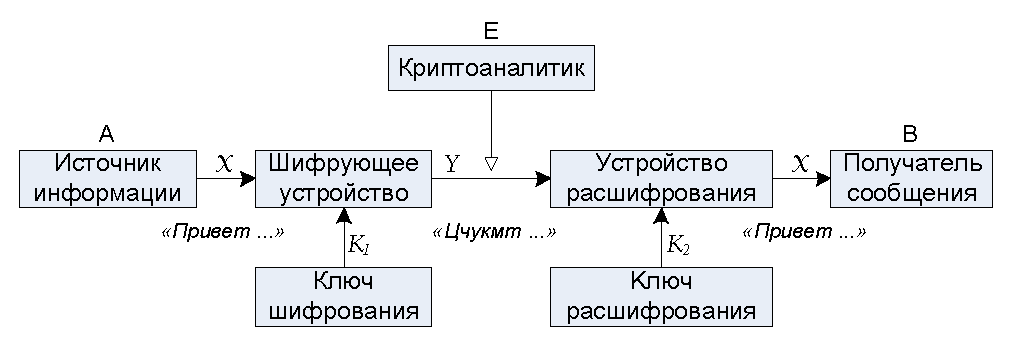
\includegraphics[width=1.0\textwidth]{pic/scheme-of-cipher}
	\caption{Передача информации с криптозащитой\label{pic:Encrypt}}
\end{figure}

\emph{Шифр}\index{шифр} -- это множество обратимых функций отображения $E_{K_1}$\index{функция!шифрования} множества открытых текстов $\set{M}$ на множество шифротекстов $\set{C}$, зависящих от выбранного ключа шифрования $K_1$ из множества $\set{K}_E$:
%обратимое отображение пары из элемента множества открытых текстов $\set{M}$ и элемента множества ключей шифрования $\set{K}_E$ в множество шифротекстов $\set{C}$:
\begin{equation}
    \label{eq:Encryption}
    Y = E_{K_1}(X), ~ X \in \set{M}, ~ K_1 \in \set{K}_E, ~ Y \in \set{C}.
\end{equation}
Можно сказать, что шифрование -- это обратимая функция двух аргументов: сообщения и ключа. Для каждого $K_1$ эта функция должна быть обратимой. Обратимость -- основное условие шифрования, по которому каждому зашифрованному сообщению $Y$ и ключу $K$ соответствует одно исходное сообщение $X$. Легальный пользователь $B$ (на приемной стороне системы связи)  получает сообщение $Y$ и осуществляет процедуру \emph{расшифрования}\index{расшифрование}.
Следует отличать шифрование от кодирования, так как кодирование -- это процесс сопоставления конкретным сообщениям строго определенной комбинации символов или сигналов, с целью повышения помехоустойчивости передаваемого сигнала.
Расшифрование --  это отображение множества шифротекстов $\set{C}$ на множество открытых текстов $\set{M}$ функцией $D_{K_2}$\index{функция!расшифрования}, зависящей от ключа расшифрования $K_2$ из множества $\set{K}_D$, являющейся обратной к функции $E_{K_1}$.
\begin{equation}
    \label{eq:Decryption}
    D_{K_2}(Y) = X, ~ Y \in \set{C}, ~ K_2 \in \set{K}_D, ~ X \in \set{M}.
\end{equation}

%Система передачи информации с криптозащитой называется \emph{криптосистемой}\index{криптосистема}.(?????)

%В общем случае функция шифрования сюръективна и псевдослучайна, отображая один открытый текст в разные шифротексты. Если функция шифрования биективна, на практике ее инкапсулируют в другую функцию с целью добиться псевдослучайности шифрования одинаковых открытых текстов в разные шифротексты.

%Методы защиты информации зависят от возможных сценариев передачи. Рассмотрим несколько основных вариантов.
Рассмотрим возможные сценарии вмешательства криптоаналитика и организации защиты информации от его действий.
Пусть  $A$ --  источник и $B$ -- получатель сообщений.

\begin{description}
    \item[Сценарий 1.] Пусть $E$ -- \emph{пассивный} криптоаналитик\index{криптоаналитик!пассивный}, который может подслушивать передачу, но не может вмешиваться в процесс передачи. Из пассивности криптоаналитика следует, что $Y = \widetilde{Y}$, и \emph{целостность} информации обеспечена.

Цель защиты --- \emph{обеспечение конфиденциальности}.

Средства защиты -- шифрование с помощью \emph{симметричных} или \emph{асимметричных } криптосистем.

Дополнительные задачи -- при большом числе пользователей должна быть решена задача \emph{генерации и доставки секретных ключей} всем пользователям.

    \item[Сценарий 2.] Пусть $E$ -- \emph{активный} криптоаналитик\index{криптоаналитик!активный}, который может изменять, удалять и вставлять сообщения или их части.

    Цель защиты -- \emph{обеспечение конфиденциальности} и  \emph{обеспечение целостности}.

Средства защиты --  шифрование и добавление \emph{имитовставки}\index{имитовставка} (message authentication code -- $\MAC$), позволяющего обнаружить нарушение целостности.

    \item[Сценарий 3.] Пусть $E$ -- активный криптоаналитик, который может изменять, удалять и вставлять сообщения или их части, дополнительно к этому легальные пользователи $A$ и $B$ не доверяют друг другу.

Цель защиты -- \emph{аутентификация} пользователей и документов.

Средства -- \emph{электронная подпись} и протокол идентификации (аутентификации) пользователей.
\end{description}

%%Возможно вмешательство нелегального пользователя $E$, называемого \emph{криптоаналитиком}.
%%
%%
%%Если $X = \widetilde{X}$, то вмешательство криптоаналитика  $E$ не изменило передаваемое сообщение, и \emph{целостность} информации обеспечена. Если криптоаналитик не получил информацию, содержащуюся в сообщении, то обеспечена \emph{конфиденциальность}.
%%
%%Если в этой системе возможна двусторонняя передача, то есть от $A$ к $B$ и от $B$ к $A$, то говорят о взаимном обмене информацией между легальными пользователями.
%
%Секретность информации в современных шифрах обеспечивается секретным ключом, в то время как сам алгоритм криптосистемы является общеизвестным. Исторический опыт, например, система шифрования A5/1 в GSM, показывает, что секретность алгоритма шифрования \emph{ослабляет} криптостойкость шифра, а не увеличивает, из-за того, что система становится малоизученной.


\section{Классификация криптосистем}

\subsection{Симметричные и асимметричные криптосистемы}
\selectlanguage{russian}

Криптографические системы и шифры можно разделить на две больших группы, в зависимости от принципа использования ключей для шифрования и расшифрования.

Если для шифрования и расшифрования используется один и тот же ключ $K$, либо если получение ключа расшифрования $K_2$ из ключа шифрования $K_1$ является тривиальной операцией, то такая криптосистема называется \textbf{симметричной}\index{криптосистема!симметричная}. В зависимости от объёма обработки данных за одну операцию шифрования симметричные шифры делятся на \textbf{блочные}\index{шифр!блочный}, в которых за одну операцию шифрования происходит преобразование одного блока данных (32 бита, 64, 128 или больше) и \textbf{потоковые}\index{шифр!потоковый}, в которых работают с каждым символом открытого текста по отдельности (например, с 1 битом или 1 байтом). Примеры блочных шифров рассмотрены в главе~\ref{chapter-block-ciphers}, а потоковых -- в главе~\ref{chapter-stream-ciphers}.

Шифрование блочным шифром подразумевает разделение открытого текста на блоки одинаковой длины. Блоки шифруются последовательно, причём результат шифрования следующего блока может зависеть от предыдущего. Это регулируется \textbf{режимом сцепления блоков}. Примеры нескольких таких режимов рассмотрены в разделе~\ref{chapter-block-chaining}.

Если ключ расшифрования получить из ключа шифрования сложно (или невозможно), то такие криптосистемы называют криптосистемами \textbf{с открытым ключом}\index{криптосистема!с открытым ключом} или \textbf{асимметричными} криптосистемами\index{криптосистема!асимметричная}. Некоторые из них рассмотрены в главе~\ref{chapter-public-key}. Все используемые на сегодняшний день асимметричные криптосистемы работают с блоком данных открытого текста, представленным в виде числа длиной в несколько сот или тысяч бит, поэтому классификация таких систем по объёму обрабатываемых за одну операцию данных не производится.

Алгоритм, который выполняет отображение аргумента произвольной длины в значение фиксированной длины, называется \textbf{хеш-функцией}. Если для такой хеш-функции выполняются определённые свойства устойчивости к поиску коллизий, то это уже \textbf{криптографическая хеш-функция}. Такие функции рассмотрены в главе~\ref{chapter-hash-functions}. Криптографические хеш-функции используются для проверки целостности сообщений. Для проверки с использованием общего секретного ключа отправителя и получателя используется механизм \textbf{имитовставки}, рассмотренный в разделе~\ref{section-MAC}. Её аналогом в криптосистемах с открытым ключом является \textbf{электронная подпись}, алгоритмы генерации и проверки которой рассмотрены в главе~\ref{chapter-public-key}, вместе с алгоритмами асимметричного шифрования.


\subsection{Шифры замены и перестановки}

Шифры по способу преобразования открытого текста в шифротекст разделяются на шифры замены и шифры перестановки.

\subsubsection{Шифры замены}
\selectlanguage{russian}

В шифрах \textbf{замены} символы одного алфавита заменяются символами другого алфавита обратимым преобразованием. В последовательности открытого текста символы входного алфавита заменяются на символы выходного алфавита. Такие шифры применяются как в симметричных системах, так и в асимметричных криптосистемах. Если при преобразовании используются однозначные функции, то шифры замены называются однозначными шифрами замены. Если используются многозначные функции, то шифры называются многозначными шифрами замены (омофонами).

В \textbf{омофоне}\index{омофон} символам входного алфавита ставится в соответствие непересекающиеся подмножества символов выходного алфавита. Количество символов в каждом подмножестве замены пропорционально частоте встречаемости символа открытого текста. Таким образом, омофон создает равномерное распределение символов шифротекста и прямой частотный криптоанализ не возможен. При шифровании омофонами символ входного алфавита заменяется на случайно выбранный из подмножества замены.

Шифры бывают \textbf{моноалфавитные}, когда для шифрования используется одно отображение входного алфавита в выходной алфавит. Если алфавит на входе и выходе одинаков и его размер (число символов) равен $D$, тогда количество всевозможных моноалфавитных шифров замены такого типа равно $D!$.

\textbf{Полиалфавитный} шифр задается множеством различных вариантов отображения входного алфавита на выходной алфавит. Шифры замены могут быть как потоковыми, так и блоковыми. Однозначный полиалфавитный потоковый шифр замены называется \textbf{шифром гаммирования}\index{шифр!гаммирования}. Символом алфавита может быть, например, 256-битовое слово, а размер алфавита -- $2^{256}$, соответственно.


\subsubsection{Шифры перестановки}

Шифры \textbf{перестановки} реализуются следующим образом. Берут открытый текст, например буквенный, и разделяют на блоки  определенной длины $x_1, x_2, \dots, x_m$. Затем осуществляется перестановка позиций блока (вместе с символами). Перестановки могут быть однократные и многократные. Частный случай перестановки -- сдвиг. Приведем пример:
\begin{center}
    секрет $\xrightarrow{\text{сдвиг}}$ ретсек $\xrightarrow{\text{перестановка}}$ рскете.
\end{center}
Ключ такого шифра указывает  изменение порядка номеров  позиций блока  при  шифровании и  расшифровании.

Существуют так называемые \textbf{маршрутные перестановки}. Используется какая-либо геометрическая фигура, например, прямоугольник. Запись открытого текста ведется по одному \emph{маршруту}, например по строкам, а считывание для шифрования осуществляется по другому маршруту, например по столбцам. Ключ шифра определяет эти маршруты.
В случае, когда рассматривается перестановка блока текста фиксированной длины, перестановку можно рассматривать как замену.

В полиалфавитных шифрах при шифровании открытый текст разбивается на блоки (последовательности) длины $n$, где $n$ -- \textbf{период}. Этот параметр выбирает \emph{криптограф} и держит его в секрете.

Поясним процедуру шифрования полиалфавитным шифром. Запишем шифруемое сообщение  в  матрицу по столбцам определенной длины. Пусть открытый текст таков: <<Игры различаются по содержанию, характерным особенностям, а также по тому, какое место они занимают в жизни детей>>. Зададим $n=4$ и запишем этот текст в  матрицу размера $(4 \times 24)$:

\begin{center} \resizebox{\textwidth}{!}{ \begin{tabular}{|c|c|c|c|c|c|c|c|c|c|c|c|c|c|c|c|c|c|c|c|c|c|c|c|}
    \hline
    и&р&и&т&о&е&н&а&т&ы&о&н&я&а&п&м&к&е&о&а&а&ж&и&е \\
    г&а&ч&с&с&р&и&р&е&м&б&о&м&к&о&у&о&с&н&н&ю&и&д&й \\
    р&з&а&о&ж&р&ю&а&р&о&е&с&а&ж&т&к&е&т&и&и&т&з&е& \\
    ы&л&ю&п&д&а&х&к&н&с&н&т&т&е&о&а&м&о&з&м&в&н&т& \\
    \hline
\end{tabular} } \end{center}

Выбираем $4$ различных моноалфавитных шифра.

Первую строку

\begin{center} \resizebox{\textwidth}{!}{ \begin{tabular}{|c|c|c|c|c|c|c|c|c|c|c|c|c|c|c|c|c|c|c|c|c|c|c|c|}
    \hline
    и&р&и&т&о&е&н&а&т&ы&о&н&я&а&п&м&к&е&о&а&а&ж&и&е \\
    \hline
\end{tabular} } \end{center}

 шифруем, используя первый шифр. Вторую строку

\begin{center} \resizebox{\textwidth}{!}{ \begin{tabular}{|c|c|c|c|c|c|c|c|c|c|c|c|c|c|c|c|c|c|c|c|c|c|c|c|}
    \hline
    г&а&ч&с&с&р&и&р&е&м&б&о&м&к&о&у&о&с&н&н&ю&и&д&й \\
    \hline
\end{tabular} } \end{center}

шифруем, используя второй шифр, и т.д.

Выполняя расшифрование, легальный пользователь знает период. Он записывает принятую шифрограмму по строкам в матрицу с длиной строки, равной периоду, и к каждому столбцу применяет соответствующий ключ и расшифровывает сообщение, зная соответствующие шифры.

Шифры перестановки можно рассматривать как частный случай шифров замены, если отождествить один блок перестановки с одним символом большого алфавита.


\subsubsection{Композиционные шифры}
\selectlanguage{russian}

Почти все современные шифры являются \emph{композиционными}~\cite{AlZKCh:2001}. Также распространено название \emph{составные шифры}, впервые введенное в работе Клода Шеннона (\langen{Claude Elwood Shannon},~\cite{Shannon:1949:CTS}). В них применяются несколько различных методов шифрования к одному и тому же открытому тексту. В современных криптосистемах используется,например, композиция шифра замены и шифра перестановок, применяемая многократно.


\subsection{Примеры современных криптографических примитивов}

Приведём примеры названий некоторых современных криптографических примитивов, из которых строят системы защиты информации:
\begin{itemize}
    \item DES\index{шифр!DES}, AES, ГОСТ 28147-89, Blowfish\index{шифр!Blowfish}, RC5\index{шифр!RC5}, RC6\index{шифр!RC6} -- блочные симметричные шифры, скорость обработки -- десятки мегабайт в секунду;
    \item A5/1, A5/2, A5/3\index{шифр!A5}, RC4\index{шифр!RC4} -- потоковые симметричные шифры с высокой скоростью, семейство A5 применяется в мобильной связи GSM, RC4 -- в компьютерных сетях для SSL-соединения между браузером и веб-сервером;
    \item RSA\index{шифр!RSA} -- криптосистема с открытым ключом для шифрования;
    \item RSA\index{электронная подпись!RSA}, DSA\index{электронная подпись!DSA}, ГОСТ Р 34.10-2001\index{электронная подпись!ГОСТ Р 34.10-2001} -- криптосистемы с открытым ключом для электронной подписи;
    \item MD5\index{хэш-функция!MD5}, SHA-1\index{хэш-функция!SHA-1}, SHA-2\index{хэш-функция!SHA-2}, ГОСТ Р 34.11-94\index{хэш-функция!ГОСТ Р 34.11-94} -- криптографические хэш-функции.
\end{itemize}

\section{Методы криптоанализа и типы атак}
\selectlanguage{russian}

Нелегальный пользователь-криптоаналитик получает информацию путём дешифрования. Сложность этой процедуры определяется числом стандартных операций, которые надо выполнить для достижения цели. \emph{Двоичной сложностью}\index{сложность!двоичная} (или битовой сложностью) алгоритма называется количество двоичных операций, которые необходимо выполнить для его завершения.
% Наиболее сложным является дешифрование полиалфавитных шифров.

Рассмотрим основные сценарии работы криптоаналитика $E$. В первом сценарии криптоаналитик может осуществлять подслушивание и (или) перехват сообщений. Его вмешательство не нарушает целостности информации: $Y=\widetilde{Y}$. Эта роль криптоаналитика называется \emph{пассивной}. Так как он получает доступ к информации, то здесь нарушается конфиденциальность.

Во втором сценарии роль криптоаналитика \emph{активная}. Он может подслушивать, перехватывать сообщения и преобразовывать их по своему усмотрению: задерживать, искажать с помощью перестановок пакетов, устраивать обрыв связи, создавать новые сообщения и т.~п. В этом случае выполняется условие $Y \neq \widetilde{Y}$. Это значит, что одновременно нарушается целостность и конфиденциальность передаваемой информации.

Приведём примеры пассивных и активных атак:
\begin{itemize}
    \item Атака <<\emph{человек посередине}>>\index{атака!<<человек посередине>>} (\langen{man-in-the-middle}) подразумевает криптоаналитика, который разрывает канал связи, встраиваясь между $A$ и $B$, получает сообщения от $A$ и от $B$, а от себя отправляет новые, фальсифицированные сообщения. В результате $A$ и $B$ не замечают, что общаются с $E$, а не друг с другом.
    \item Атака \emph{воспроизведения}\index{атака!воспроизведения} (\langen{replay attack}) предполагает, что криптоаналитик может записывать и воспроизводить шифротексты, имитируя легального пользователя.
    \item Атака на \emph{различение} сообщений\index{атака!на различение} означает, что криптоаналитик, наблюдая одинаковые шифротексты, может извлечь информацию об идентичности исходных открытых текстов.
    \item Атака на \emph{расширение} сообщений\index{атака!на расширение} означает, что криптоаналитик может дополнить шифротекст осмысленной информацией без знания секретного ключа.
    \item \emph{Фальсификация} шифротекстов\index{атака!фальсификацией} криптоаналитиком без знания секретного ключа.
\end{itemize}

Часто для нахождения секретного ключа криптоатаки строят в предположениях о доступности дополнительной информации. Приведём примеры:
\begin{itemize}
    \item Атака на основе известного открытого текста\index{атака!с известным открытым текстом} (\langen{chosen plaintext attack, CPA}) предполагает, что криптоаналитик имеет возможность выбирать открытый текст и получать для него соответствующий шифротекст.
    \item Атака на основе известного шифротекста\index{атака!с известным шифротекстом} (\langen{chosen ciphertext attack, CCA}) предполагает возможность криптоаналитику выбирать шифротекст и получать для него соответствующий открытый текст.
\end{itemize}

Обязательным требованием к современным криптосистемам является устойчивость ко всем известным типам атак: пассивным, активным и с дополнительной информацией.


%Приведём примеры возможных вариантов работы активного криптоаналитика.
%\begin{itemize}
%\item Криптоаналитик имеет $m$ шифрованных сообщений $Y_{1},Y_{2},\ldots Y_{m}$ и пытается определить ключ или прочитать открытый текст $X_{1},X_{2},\ldots X_{m}.$
%\item Криптоаналитик имеет несколько пар открытого и шифрованного текстов
%
%$(Y_{1},X_{1}),(Y_{2}X_{2}),\ldots (Y_{m}X_{m})$ и пытается дешифровать остальной текст или определить алгоритм шифрования или определить ключ.
%\item
%\item
%\item
%\end{itemize}

Для защиты информации от активного криптоаналитика и обеспечения её целостности дополнительно к шифрованию сообщений применяют имитовставку\index{имитовставка}. Для неё используют обозначение $\MAC$ (\langen{message authentication code}). Как правило, $\MAC$ строится на основе хэш-функций, которые будут описаны далее.

Существуют ситуации, когда пользователи $A$ и $B$ не доверяют друг другу. Например, $A$ -- банк, $B$ -- получатель денег. $A$ утверждает, что деньги переведены, $B$ утверждает, что не переведены. Решение задачи аутентификации и неотрицаемости состоит в обеспечении \emph{электронной подписью}\index{электронная подпись} каждого из абонентов. Предварительно надо решить задачу о генерировании и распределении секретных ключей.

В общем случае, системы защиты информации должны обеспечивать:
\begin{itemize}
    \item конфиденциальность\index{конфиденциальность} (защита от наблюдения);
    \item целостность\index{целостность} (защита от изменения);
    \item аутентификацию (защита от фальсификации пользователя и сообщений);
    \item доказательство авторства информации (доказательство авторства и защита от его отрицания).
\end{itemize}
как со стороны получателя, так и со стороны отправителя.

Важным критерием для выбора степени защиты является сравнение стоимости реализации взлома для получения информации и экономического эффекта от владения ей. Очевидно, что если стоимость взлома превышает ценность информации, взлом нецелесообразен.

%Сценарии защиты информации
%   Сценарий 1. A -- передающая сторона. B -- принимающая сторона. E -- пассивный
%криптоаналитик, который может подслушивать передачу, но не может вмешиваться
%в процесс передачи. Цель защиты: обеспечение конфиденциальности. Средства
%-- методы шифрования с секретным ключом (симметричные системы шифрования)
%и методы шифрования с открытым ключом (асимметричные системы шифрования).
%Сценарий 2. E -- активный криптоаналитик, который может изменять, удалять и вставлять
%сообщения или их части. Цель защиты -- обеспечение конфиденциальности (не
%всегда) и обеспечение целостности. Средства -- методы шифрования и добавление
%имитовставки\index{имитовставка} (Message Autentication Code -- $\MAC$).
%Сценарий 3. A и B не доверяют друг другу. Цель защиты -- аутентификация пользователя.
%Средства -- электронная подпись.


\section{Минимальные длины ключей}
\selectlanguage{russian}

Оценим минимальную битовую длину ключа для обеспечения криптостойкости, то есть защиты криптосистемы от атаки, полным перебором всех возможных секретных ключей. Сделаем такие предположения:

\begin{itemize}
    \item одно ядро процессора выполняет $R = 10^7 \approx 2^{23}$ шифрований и расшифрований в секунду;
    \item вычислительная сеть состоит из $n = 10^3 \approx 2^{10}$ узлов;
    \item в каждом узле имеется $C = 16 = 2^4$ ядер процессора;
    \item нужно обеспечить защиту данных на $Y = 100$ лет, т.е. на $S \approx 2^{32}$ с;
    \item выполняется закон Мура об удвоении вычислительной производительности на единицу стоимости каждые 2 года, то есть производительность вырастет в $M = 2^{Y/2} \approx 2^{50}$ раз.
\end{itemize}

Число переборов $N$ примерно равно
    \[ N \approx R \cdot n \cdot C \cdot S \cdot M, \]
    \[ N \approx 2^{23} \cdot 2^{10} \cdot 2^{4} \cdot 2^{32} \cdot 2^{50} = 2^{23+10+4+32+50} = 2^{119}. \]

Следовательно, минимально допустимая длина ключа для защиты от атаки перебором на 100 лет составляет порядка
    \[ \log_2 N \approx 119\text{ бит} \] .

Например, в 1997 году предыдущий американский стандарт шифрования DES с 56-битовым секретным ключом впервые был взломан перебором интернет-сетью из 78 000 частных компьютеров, производивших фоновые вычисления по проекту \textsc{DesChal}.



\subimport*{historical-ciphers/}{index}

\section[Криптосистема совершенной стойкости]{Криптосистема совершенной \protect\\ стойкости}
\selectlanguage{russian}

Понятие совершенной секретности (или стойкости) введено американским ученым Клодом Шенноном. В конце Второй мировой войны он закончил работу, посвященную теории связи в секретных системах\cite{Shannon:1949:CTS}. Эта работа вошла составной частью в собрание его трудов, вышедшее в русском переводе в 1963 году \cite{Shannon:1963}. Понятие о стойкости шифров по Шеннону связано с решением задачи криптоанализа по одной криптограмме.

Криптосистемы совершенной стойкости могут применяться как в современных вычислительных сетях так и для шифрования любой бумажной корреспонденции. Основной проблемой применения данных шифров для шифрования больших объемов информации является необходимость распространения ключей объемом, не меньшим чем передаваемые сообщения.

\subsection{Условие совершенной криптостойкости}


Пусть $M$ -- множество открытых текстов, подлежащих шифрованию, $K$ -- множество ключей, $C$ -- множество зашифрованных сообщений для выбранного ключа, $A$ и $B$ -- легальные пользователи.

\textbf{Утверждается следующее}: если сообщение из $M$ и соответствующий ему шифротекст из $C$ -- статистически независимые случайные величины, то такая криптосистема обладает \textbf{совершенной криптостойкостью}.

Докажем это утверждение. Так как шифрование является однозначной функцией, то пара (шифротекст, ключ) однозначно определяет открытый текст и, следовательно, условная энтропия открытого текста равна 0:
\[H(M|K,C)=0.\]
Найдем оценку количества информации, которое содержит шифротекст $C$ относительно сообщения  $M$
\[ I(M; C) = H(M) - H(M | C). \]
Очевидны следующие соотношения условных и безусловных энтропий \cite{GabPil:2007}:
\[H(K|C)=H(K|C)+H(M|K,C)=H(M,K|C),\]
\[H(M,K|C)=H(M|C)+H(K|M,C)\geq H(M|C),\]
\[H(K)\geq H(K|C)\geq H(M|C).\]
Отсюда получаем:
 \[ I(M; C) = H(M) - H(M | C)\geq H(M)-H(K). \]
Из последнего неравенства следует, что взаимная информация между сообщением и шифротекстом равна нулю, если энтропия ключа не меньше энтропии сообщений. С другой стороны, взаимная информация между сообщением и шифротекстом равна нулю, если они статистически независимы. Таким образом условием  совершенной криптостойкости является неравенство
\[ H(M) \leq  H(K).\]
%Если утверждение верно, то количество информации в шифротексте относительно открытого текста $I(M; C)$ равно нулю:
%  \[ I(M; C) = H(M) - H(M | C) = 0, \]
%так как для статистически независимых величин условная энтропия равна безусловной энтропии, то есть $H(M) = H(M | C)$.

%Функцию шифрования обозначим $E: \{ M, K \} \rightarrow C$. Процедура шифрования состоит из следующих шагов.
%\begin{itemize}
%    \item Легальный пользователь $A$ выбирает ключ $k \in K$ и секретно сообщает его легальному пользователю $B$ (дополнительная задача -- распределение ключей).
%    \item По открытому сообщению $m \in M$ и выбранному ключу $k$ вычисляют шифрованное сообщение $c = E_k(m) \in C$.
%\end{itemize}

%Основное требование при шифровании состоит в том, чтобы при выбранном ключе $k$ вычисление $c$  было легкой задачей для любого сообщения $m$.

%Функцию расшифрования обозначим $D: \{ C, K \} \rightarrow M$.  Процедура расшифрования состоит из следующих шагов.
%\begin{itemize}
%    \item Легальный пользователь $B$ получает от $A$ секретный ключ $k \in K$.
 %   \item $B$ по принятому шифрованному сообщению $c \in C$ и известному  ключу $k$ вычисляет открытое сообщение $m = D_k(c) \in M$.
%\end{itemize}

%Основное требование: при выбранном ключе $k$ вычисление $m$ должно быть легкой задачей для любого $c$. С другой стороны, при неизвестном ключе $k$ вычисление открытого сообщения $m$ по известному шифрованному сообщению $c$ должно быть трудной задачей для любого $c$.

%Криптостойкость шифра оценивается числом операций, необходимым для определения: открытого текста $m$ по шифротексту $c$, либо ключа шифрования $k$ по открытому тексту $m$ и шифротексту $c$.

%$M, C, K$ интерпретируются как случайные величины.
%Пусть заданы  распределения вероятностей $P_m(M), P_c(C), P_k(K)$. По определению шифрование $C = E_K(M)$ -- детерминированная функция своих аргументов.
%Если при выбранном шифре оказалось, что открытый текст $M$ и шифротекст $C$ -- статистически независимые случайные величины, то считается, что такая система обладает совершенной криптостойкостью.


%\subsection{Длина ключа}

%Пусть сообщения $m\in M$ и ключи $r\in K$ являются независимыми случайными величинами. Это значит, что их совместная вероятность $P_{mk}(M, K)$ равна произведению отдельных вероятностей:
%\[P_{mk}(M, K) = P_m(M) \cdot P_k(K).\]
%Пусть $C = E_K(M)$ -- множество шифрованных текстов, $M = D_K(C)$ -- множество расшифрованных текстов. Можно найти вероятности $P_c(C), P_{mck}(M,C,K)$.

%Используя известные соотношения о безусловной и условной энтропии~\cite{GabPil:2007}, оценим энтропию открытых текстов $M$ с учетом статистической независимости $M$ и $C$:
 %   \[ H(M) = H(M | C) \leq H(MK | C) = H(K | C) + H(M | CK) = \]     \[ = H(K | C) \leq H(K). \]

%Так как энтропия открытого текста при заданном шифротексте и известном ключе равна нулю, то $H(M|CK)=0$.  В результате получаем     \[ H(M) \leq H(K). \]

Обозначим $L(M)$ и $L(K)$ длину сообщений и ключа, соответственно. Известно~\cite{GabPil:2007}, что $H(M)\leq L(M)$ и равенство достигается, когда сообщения состоят из статистически независимых и равновероятных символов. Такое же свойство выполняется и для случайных ключей $H(K)\leq L(K)$. Таким образом, достаточным условием совершенной криптостойкости системы можно считать неравенство
 \[ L(M) \leq L(K)\]
при случайном выборе ключа.

%С другой стороны, энтропия открытого текста $H(M)$ характеризует  длину последовательности для описания случайной величины $M$ (открытого сообщения), а $H(K)$ характеризует  длину последовательности для описания ключа. Следовательно, совершенная криптостойкость возможна только тогда, когда  длина ключа не меньше, чем длина шифруемого сообщения, то есть     \[ H(M) \leq H(K). \] Как правило, длина сообщения заранее неизвестна и ограничена большим числом. Выбрать ключ длины не меньшей, чем возможное сообщение не представляется возможным или рациональным, и один и тот же ключ (или его преобразования) используется многократно для шифрования блоков сообщения фиксированной длины. То есть, $H(K) \ll H(M)$.

На самом деле, сообщение может иметь произвольную (заранее не ограниченную) длину. Поэтому генерация и, главным образом, доставка легальным пользователям случайного и достаточного длинного ключа становятся критическими проблемами. Практическим решением этих проблем является многократное использование одного и того же ключа при условии, что его длина гарантирует вычислительную невозможность любой известной атаки на подбор ключа.


\subsection{Криптосистема Вернама}

Приведем пример системы с совершенной криптостойкостью.

Пусть сообщение представлено двоичной последовательностью длины $N$:
    \[ m = (m_1, m_2, \dots, m_N). \]
Распределение вероятностей сообщений $P_m(m)$ может быть любым.  Ключ также представлен двоичной последовательностью $ k = (k_1, k_2, \dots, k_N)$ той же длины, но с равномерным распределением
    \[ P_k(k) = \frac{1}{2^N} \]
для всех ключей.

Шифрование в криптосистеме \textbf{Вернама} осуществляется путем покомпонентного суммирования по модулю алфавита последовательностей открытого текста и ключа:
    \[ C = M \oplus K = (m_1 \oplus k_1, ~ m_2 \oplus k_2, \dots,  m_N \oplus k_N). \]

Легальный пользователь знает ключ и осуществляет расшифрование:
    \[ M =C \oplus K = (m_1 \oplus k_1, ~ m_2 \oplus k_2, \dots, m_N \oplus k_N). \]

Найдем вероятностное распределение $N$-блоков шифротекстов, используя формулу
    \[ P(c = a) = P(m \oplus k = a) = \sum_{m} P(m) P(m \oplus k = a | m) = \]
    \[ = \sum_{m} P(m) P(k \oplus m) = \sum_{m} P(m) \frac{1}{2^N} = \frac{1}{2^N}. \]

Получили подтверждение известного факта: сумма двух случайных величин, одна из которых  имеет равномерное распределение, является случайной величиной с равномерным распределением. В нашем случае распределение ключей  равномерное, поэтому распределение шифротекстов тоже равномерное.

Запишем совместное распределение открытых текстов и шифротекстов:
    \[ P(m = a, c = b) ~=~ P(m = a) ~ P(c = b | m = a). \]

Найдем условное распределение
    \[ P(c = b | m = a) ~=~ P(m \oplus k = b | m = a) ~= \]
    \[ =~ P(k = b \oplus a | m = a) ~=~ P(k = b \oplus a) ~=~ \frac{1}{2^N}, \]
так как ключ и открытый текст являются независимыми случайными величинами. Итого:
    \[ P(c=b | m=a) = \frac{1}{2^N}. \]

Подстановка правой части этой формулы в формулу для совместного распределения дает
    \[ P(m=a,c=b)=P(m=a)\frac{1}{2^N}, \]
что доказывает независимость шифротекстов и открытых текстов в этой системе. По доказанному выше количество информации в шифротексте относительно открытого текста равно нулю. Это значит, что рассмотренная криптосистема Вернама обладает совершенной секретностью (криптостойкостью) при условии, что для каждого $N$-блока (сообщения) генерируется случайный (одноразовый) $N$-ключ.


\subsection{Расстояние единственности}

В реальной ситуации длина ключа может быть меньше длины открытого текста, поскольку передача ключа при больших объемах текста будет затруднена большим объемом ключа.  Это означает, что энтропия ключа может быть меньше энтропии открытого текста: $H(K)< H(M)$. Для таких ситуаций важным понятием является \textbf{расстояние единственности}.

Пусть шифрованное сообщение $C$ состоит из $N$ символов алфавита, состоящего из $L$ букв:
\[
    C = (C_1, C_2, \dots, C_N).
\]
Пусть символы этой последовательности выбираются случайно и независимо из заданного алфавита.

Криптоаналитик теоретически может вычислить последовательность энтропий:
\[ \begin{array}{l}
    h_0 = H(K), \\
    h_1 = H(K | C_1), \\
    h_2 = H(K | C_1, C_2), \\
    \dots \\
    h_n = H(K | C_1, C_2, \dots, C_n), \\
    \dots
\end{array} \]

Функция $h_n$ называется \emph{функцией неопределенности ключа}. Она является невозрастающей функцией числа условных величин $n$. Если для некоторого значения $n = n_u$ окажется, что $h_{n_u} = 0$, то это будет означать, что ключ $K$ является детерминированной функцией первых $n_u$ случайных величин $C_1, C_2, \dots, C_{n_u}$ и при неограниченных вычислительных возможностях может быть вычислен. Число $n_u$ называется \emph{расстоянием единственности}.

Найдем типичное поведение функции $h_n$ и значение расстояния единственности $n_u$. Используем следующие предположения.
\begin{itemize}
    \item Криптограф всегда стремится спроектировать систему таким образом, чтобы символы шифрованного текста имели равномерное распределение и, следовательно, энтропия шифротекста имела максимальное значение:
            \[ H(C_1 C_2 \dots C_n) \approx n \log_2 L, ~ n = 1, 2, \dots, N. \]
    \item Имеет место соотношение
            \[ H(C | K) = H(C_1 C_2 \dots C_N | K)  =  H(M), \]
        которое следует из цепочки равенств
            \[ H(MCK) = H(M) + H(K | M) + H(C | MK) = H(M) + H(K), \]
        так как
            \[ H(K | M) = H(K), ~~ H(C | MK) = 0, \]
            \[H(MCK) = H(K) + H(C | K) + H(M | CK) = H(K) + H(C | K), \]
        поскольку
            \[ H(M | CK) = 0, \]
            \[ H(C | K) =  H(M). \]
    \item Предполагается, что для любого $n \le N$ приближенно выполняется соотношение
        \[ H(C_n | K) \approx \frac{1}{N} H(M), \]
        \[ H(C_1 C_2\dots C_n | K) \approx \frac{n}{N} H(M). \]
\end{itemize}

Вычислим энтропию $H(C_1 C_2 \dots C_n K)$ двумя способами:
    \[ H(C_1 C_2 \dots C_n K) = H(C_1 C_2 \dots C_n) + H(K | C_1 C_2 \dots C_n) \approx \]
        \[ \approx n \log_2 L + h_n, \]
    \[H(C_1 C_2 \dots C_n K) = H(K) + H(C_1 C_2 \dots C_n | K) \approx \]
        \[ \approx H(K) + \frac{n}{N} H(M). \]

Отсюда следует, что
    \[ h_n \approx H(K) + n \left( \frac{H(M)}{N} - \log_2 L \right) \]
и
    \[ n_u = \frac{H(K)}{ \left( 1 - \frac{H(M)}{N \log_2 L} \right) \log_2 L} = \frac{H(K)}{\rho \log_2 L}. \]
Здесь
    \[ \rho = 1 - \frac{H(M)}{N \log_2 L} \]
означает избыточность источника открытых текстов.

%Минимальное $n$, при котором накопленная избыточность текста превысит энтропию ключа
%    \[ \frac{n}{N} H(M) = H(K), \]
%    \[ n = N \frac{H(K)}{H(M)}. \]

Несмотря на то, что теоретический вывод о совершенной криптостойкости для практики не приемлем, так как требует большого объема ключа, сравнимого с объемом открытого текста, разработанные идеи находят успешное применение в современных криптосистемах. Вытекающий из идей Шеннона принцип  выравнивания апостериорного распределения символов в шифротекстах используется в современных криптосистемах с помощью многократных итераций, включающих замены и перестановки.


\subimport*{block-ciphers/}{index}

\chapter{Генераторы псевдослучайных чисел}\label{chapter-generators}
\selectlanguage{russian}

Для работы многих криптографических примитивов необходимо уметь получать случайные числа:
\begin{itemize}
	\item вектор инициализации для отдельных режимов сцепления блоков должен быть случайным числом (см. раздел~\ref{section-block-chaining});
	\item для генерации пар открытых и закрытых ключей необходимы случайные числа (см. главу~\ref{chapter-public-key});
	\item стойкость многих протоколов распределения ключей (см. главу~\ref{chapter-key-distribution-protocols}) основывается в том числе на выработке случайных чисел (\langen{nonce}), которые не может предугадать злоумышленник.
\end{itemize}

Генератором случайных чисел (\langen{random number generator})\index{генератор!случайных чисел} мы будем называть процесс\footnote{Есть и строгое математическое определение генератора в общем смысле. Генератором называется функция $g: \left\{0, 1\right\}^{n} \to \left\{0, 1\right\}^{q\left(n\right)}$, вычислимая за полиномиальное время. Однако мы пока не будем использовать это определение, чтобы показать разницу между истинно случайными числами и псевдослучайными.}, результатом работы которого является случайная последовательность чисел, а именно такая, что зная произвольное число предыдущих чисел последовательности (и способ их получения), даже теоретически нельзя предсказать следующее с вероятностью больше заданной. К таким случайным процессам можно отнести:

\begin{itemize}
	\item результат работы счётчика элементарных частиц, работа с которым включена в лабораторный практикум по общей физике для студентов первого курса МФТИ;
	\item время между нажатиями клавиш на клавиатуре персонального компьютера или расстояние, которое проходит <<мышь>> во время движения;
	\item время между двумя пакетами, полученными сетевой картой;
	\item тепловой шум, измеряемый звуковой картой на входе аналогового микрофона, даже в отсутствие самого микрофона.
\end{itemize}

Хотя для всех этих процессов можно предсказать приблизительное значение (чётное или нечётное), его последний бит будет оставаться достаточно случайным для практических целей. С учётом данной поправки их можно называть надёжными или качественными генераторами случайных чисел.

Однако к генератору случайных чисел предъявляются и другие требования. Кроме уже указанного критерия \emph{качественности} или \emph{надёжности}, генератор должен быть \emph{быстрым} и \emph{дешёвым}. Быстрым -- чтобы получить большой объём случайной информации за заданный период времени. И дешёвым -- чтобы его можно было бы использовать на практике. Количество случайной информации от перечисленных выше генераторов составляет не более десятков килобайт в секунду (для теплового шума) и значительно меньше, если мы будем требовать ещё и равномерность распределения полученных случайных чисел.

С целью получения большего объёма случайной информации используют специальные алгоритмы, которые называют генераторами псевдослучайных чисел (ГПСЧ). ГПСЧ -- это детерминированный алгоритм, выходом которого является последовательность чисел, обладающая свойством случайности. Работу ГПСЧ можно описать следующей моделью. На подготовительном этапе оперативная память, используемая алгоритмом, заполняется начальным значением (\langen{seed}). Далее на каждой итерации своей работы ГПСЧ выдаёт на выход число, которое является функцией от состояния оперативной памяти алгоритма и меняет содержимое своей памяти по определённым правилам. Содержимое оперативной памяти называется \emph{внутренним состоянием} генератора.

Как и у любого алгоритма, у ГПСЧ есть определённый размер используемой оперативной памяти\footnote{Только алгоритмы с фиксированным размером используемой оперативной памяти и можно называть \emph{генераторами} в строгом математическом смысле этого слова, как следует из определения.}. Исходя из практических требований, предполагается, что размер оперативной памяти для ГПСЧ сильно ограничен. Так как память алгоритма ограничена, то ограничено и число различных внутренних состояний алгоритма. В силу того, что выдаваемые ГПСЧ числа являются функцией от внутреннего состояния, то любой ГПСЧ, работающий с ограниченным размером оперативной памяти и не принимающий извне дополнительной информации, будет иметь \emph{период}. Для генератора с памятью в $n$ бит максимальный период, очевидно, равен $2^n$.

Качество детерминированного алгоритма, то есть то, насколько полученная последовательность обладает свойством случайной, можно оценить с помощью тестов, таких как набор тестов NIST (\langen{National Institute of Standards and Technology}, США,~\cite{NIST:2001}). Данный набор содержит большое число различных проверок, включая частотные тесты бит и блоков, тесты максимальных последовательностей в блоке, тесты матриц и так далее.

\section{Линейный конгруэнтный генератор}\label{section-linear-congruential-generator}\index{генератор!линейный конгруэнтный}
\selectlanguage{russian}

Алгоритм был предложен Лемером (\langen{Derrick Henry Lehmer},~\cite{Lehmer:1951:1, Lehmer:1951:2}) в 1949 году. Линейный конгруэнтный генератор основывается на вычислении последовательности $x_n, x_{n+1}, \dots$, такой что:
	\[x_{n+1} = a \cdot x_n + c \mod m.\]

Числа $a, c, m$, $0 < a < m$, $0 < c < m$ являются параметрами алгоритма.

\example
Для параметров $a = 2$, $c = 3$, $m = 5$ и начального состояния $x_0 = 1$ получаем последовательность: $0, 3, 4, 0, 3, 4, \dots$
\exampleend

Максимальный период ограничен значением $m$. Но максимум периода достигается тогда и только тогда, когда~\cite[Линейный конгруэнтный метод]{Knuth:2001:2}:

\begin{itemize}
	\item числа $c$ и $m$ взаимно просты\index{числа!взаимно простые};
	\item число $a - 1$ кратно каждому простому делителю числа $m$;
	\item число $a - 1$ кратно 4, если $m$ кратно 4.
\end{itemize}

Конкретная реализация алгоритма может использовать в качестве выхода либо внутреннее состояние целиком (число $x_n$), либо его отдельные биты. Линейный конгруэнтный генератор является простым (то есть <<дешёвым>>) и быстрым генератором, результатом его работы является статистически качественная псевдослучайная последовательность. Линейный конгруэнтный генератор нашёл широкое применение в качестве стандартной реализации функции \texttt{random} в различных компиляторах и библиотеках времени исполнения (см. таблицу~\ref{table:lcg}). Но, забегая вперёд, его использование в криптографии недопустимо. Зная два последовательных значения выхода генератора ($x_n$ и $x_{n+1}$) и единственный параметр схемы $m$, можно решить систему уравнений и найти $a$ и $c$, чего будет достаточно для нахождения всей дальнейшей (или предыдущей) части последовательности. Параметр $m$, в свою очередь, можно найти перебором, начиная с некоторого $\min(X): X \geq x_i$, где $x_i$ -- наблюдаемые элементы последовательности.

\begin{landscape}
{\renewcommand{\arraystretch}{1.5}
\begin{table}[h]
\begin{tabular}{|p{0.34\linewidth}|r|r|r|l|}
\hline
									& a		& c		& m		& используемые биты	\\
\hline
\cite{Press:2007}~Numerical Recipes: The Art of Scientific Computing	& 1664525	& 1013904223	& $2^{32}$	& 			\\
\cite{Knuth:2005}~MMIX in The Art of Computer Programming & \tiny{6364136223846793005} & \tiny{1442695040888963407}	& $2^{64}$	&	\\
\hline
\cite{Entacher:1997}~ANSI C:
\tiny{(Watcom, Digital Mars, CodeWarrior, IBM VisualAge C/C++)}		& 1103515245	& 12345		& $2^{31}$	& биты с 30 по 16-й	\\
\cite{Sirca:Horvat:2012}~glibc						& 1103515245	& 12345		& $2^{31}$	& биты с 30 по 0-й	\\
C99, C11 (ISO/IEC 9899) 						& 1103515245	& 12345		& $2^{32}$	& биты с 30 по 16-й	\\
C++11 (ISO/IEC 14882:2011) 						& 16807		& 0		& $2^{31} - 1$	& 			\\
Apple CarbonLib             			                       	& 16807		& 0		& $2^{31} - 1$	& 			\\
Microsoft Visual/Quick C/C++                                    	& 214013	& 2531011	& $2^{32}$	& биты с 30 по 16-й	\\
\hline
\cite{Bucknall:2001}~Borland Delphi					& 134775813	& 1		& $2^{32}$	& \\
\cite{MS-VBRAND:2004}~Microsoft Visual Basic \tiny{(версии 1--6)}	& 1140671485	& 12820163	& $2^{24}$	& 			\\
\cite{Mak:2003}~ Sun (Oracle) Java Runtime Environment			& 25214903917	& 11		& $2^{48} - 1$	& биты с 47 по 16-й	\\
\hline
\end{tabular}
\caption{Примеры параметров линейного конгруэнтного генератора в различных книгах, компиляторах и библиотеках времени исполнения\label{table:lcg}}
\end{table}
}
\end{landscape}


\section[РСЛОС]{Регистр сдвига с линейной обратной связью}\label{section-lfsr}
\selectlanguage{russian}

Другой схемой построения псевдослучайных генераторов является использование регистров сдвига с линейной обратной связью, а также их вариациями. Для начала рассмотрим простой РСЛОС, изображённый на рисунке~\ref{fig:lfsr}.

\begin{figure}[thb]
	\centering
	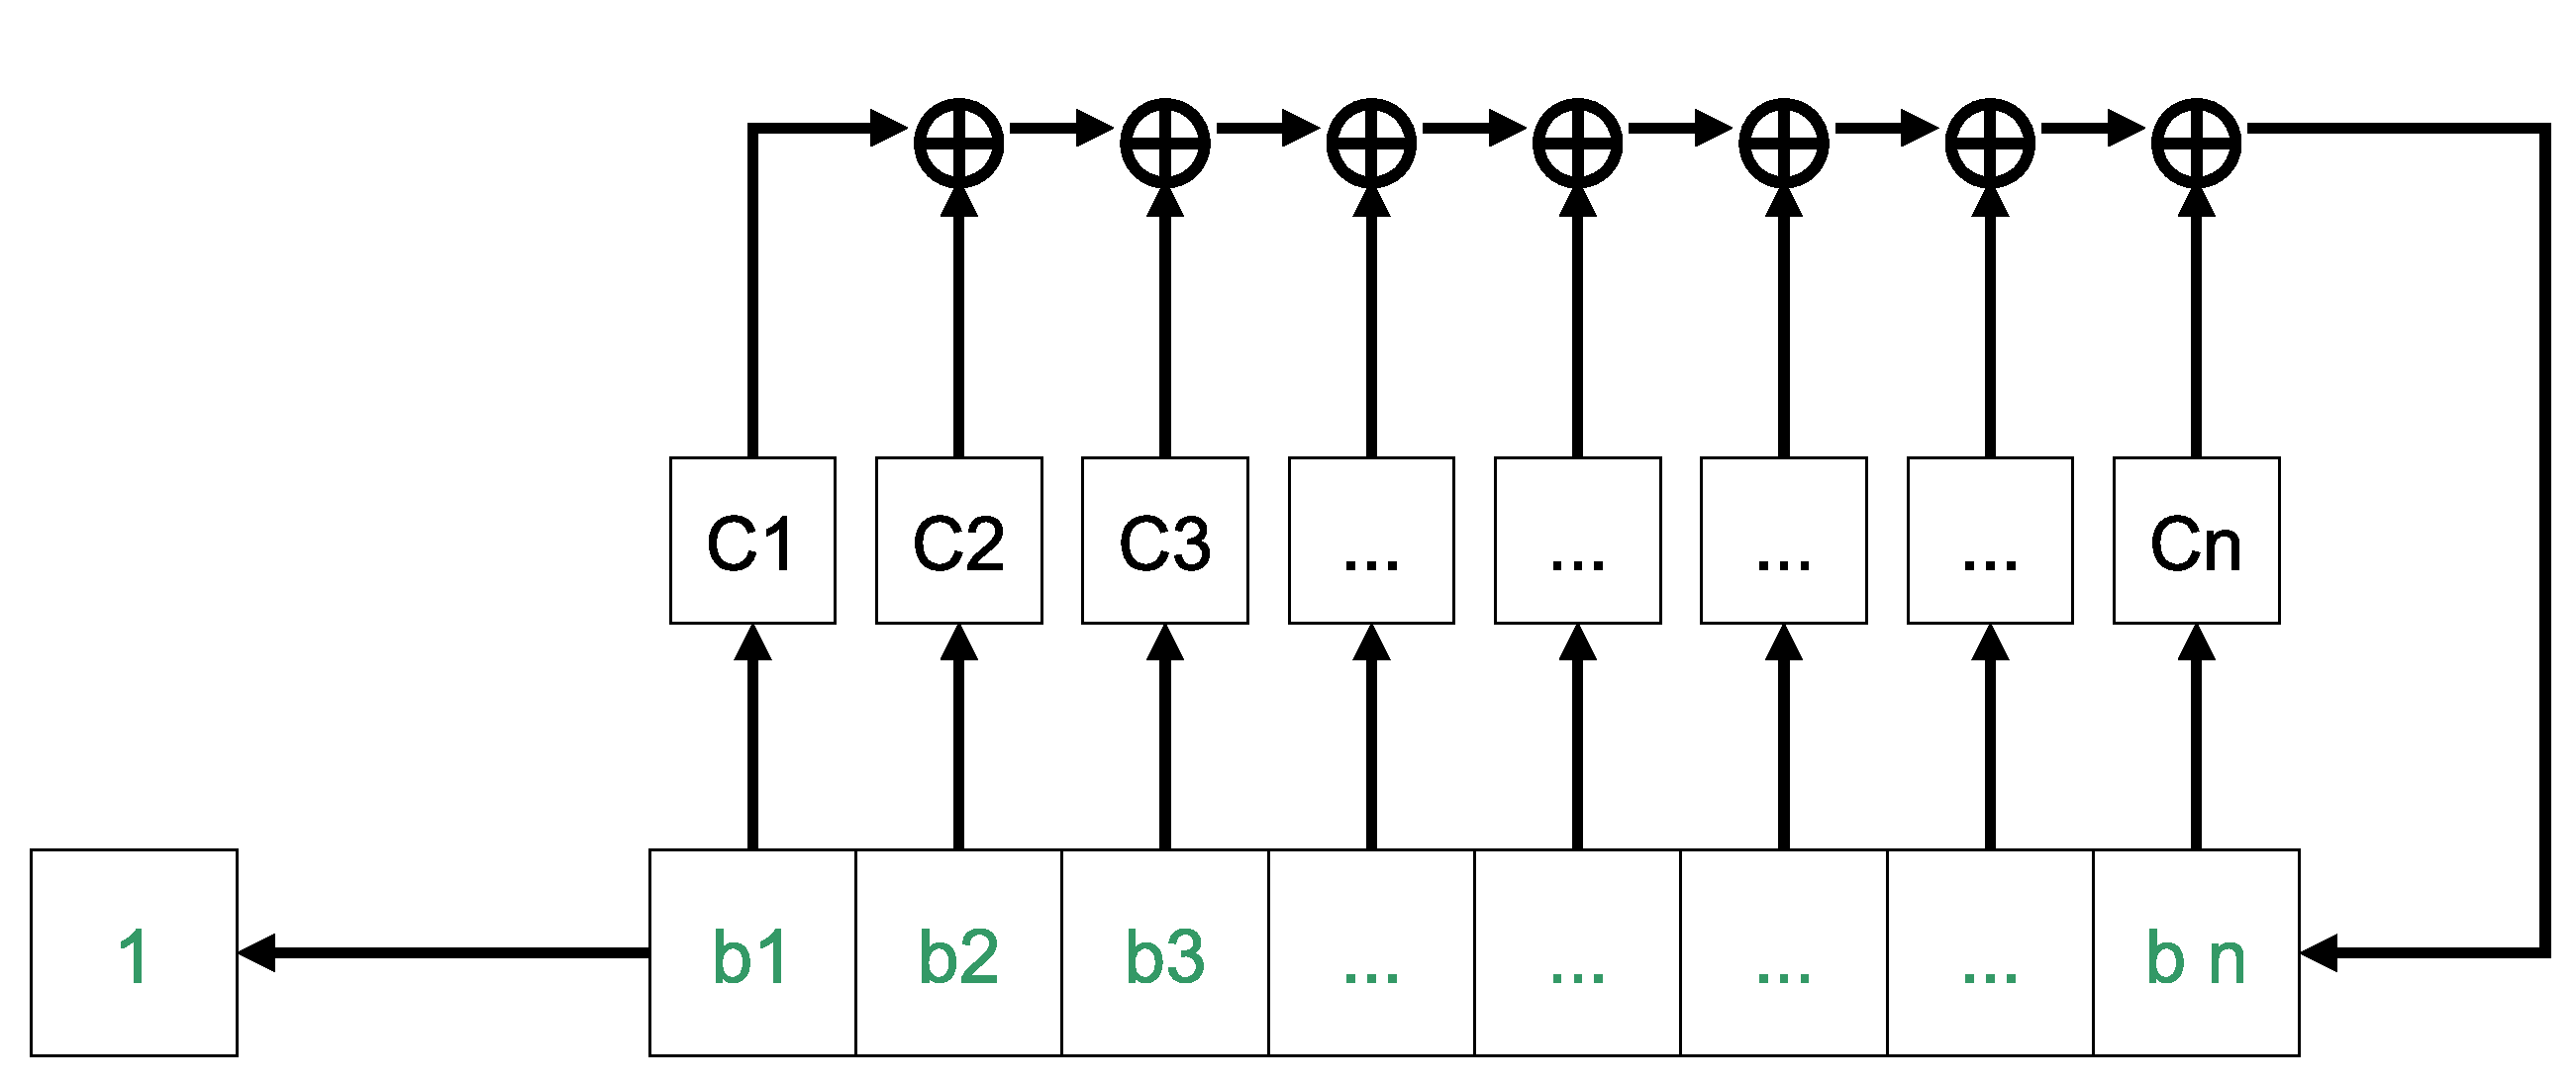
\includegraphics[width=0.75\textwidth]{pic/lfsr}
	\caption{Регистр сдвига с линейной обратной связью}
	\label{fig:lfsr}
\end{figure}

Регистр сдвига состоит из $n$ однобитовых ячеек $b_1, b_2, \dots, b_n$, содержащих 0 или 1, и линейной обратной связи, определяемой коэффициентами $C_1 = 1$, $C_2, C_3, \dots, C_n \in \{0, 1\}$. Многочлен над полем GF(2) вида $C_1 x^n + C_2 x^{n-1} + \dots + C_n x + 1$ называется характеристическим многочленом РСЛОС.

Начальным состоянием генератора является набор значений в битовых ячейках. На каждой итерации генератор вычисляет сумму по модулю два (то есть выполняет операцию XOR) значений ячеек, для которых $C_i=1$:
\[\begin{array}{ll}
	b_{n+1} &= \sum\limits_{i} C_i b_i \mod 2, \\
	b_{n+1} &= b_1 \oplus C_2 b_2 \oplus C_3 b_3 \oplus \dots \oplus C_n b_n.
\end{array}\]

Далее регистр сдвигает значения на одну ячейку влево. Самая правая ячейка $b_n$ принимает вычисленное значение $b_{n+1}$:
\[\begin{array}{ll}
	b_1 := b_2, \\
	b_2 := b_3, \\
	\dots \\
	b_n := b_{n+1}. \\
\end{array}
\]

Выходом генератора является значение ячейки $b_1$ после сдвига.

\example
Пусть регистр сдвига с линейной обратной связью задан характеристическим многочленом $m\left(x\right)=x^{5} + x^{3} + 1$. Как показано на рисунке, регистр состоит из пяти ячеек. В линейной обратной связи будут участвовать ячейки 1 и 3 (то есть $C_1 = 1, C_3 = 1$, остальные $C_i = 0$).

\begin{center}
	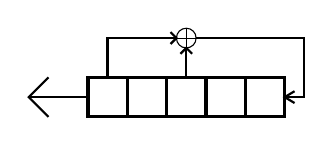
\begin{tikzpicture}[scale=0.05]
		\draw[black,very thick] (30,30) -- (30,40) -- (40,40) -- (40,30) -- (30,30) -- (30,40);
		\draw[black,thick] (35,40) -- (35,50) -- (35,50) -- (37.5,50);
		\draw[black,very thick] (40,30) -- (40,40) -- (50,40) -- (50,30) -- (40,30) -- (40,40);
		\draw[black,very thick] (50,30) -- (50,40) -- (60,40) -- (60,30) -- (50,30) -- (50,40);
		\draw[black,thick] (55,40) -- (55,47.5);
		\draw[black,thick] (53.5,46) -- (55,47.5) -- (56.5,46);
		\draw[black,thick] (37.5,50) -- (52.5,50);
		\draw[black,thick] (51,51.5) -- (52.5,50) -- (51,48.5);
		\draw (55,50) circle [radius=2.5];
		\draw[black] (52.5,50) -- (57.5,50);
		\draw[black] (55,47.5) -- (55,52.5);
		\draw[black,very thick] (60,30) -- (60,40) -- (70,40) -- (70,30) -- (60,30) -- (60,40);
		\draw[black,very thick] (70,30) -- (70,40) -- (80,40) -- (80,30) -- (70,30) -- (70,40);
		\draw[black,thick] (57.5,50) -- (85,50) -- (85,35) -- (80,35);
		\draw[black,thick] (82.5,36.5) -- (80,35) -- (82.5,33.5);
		\draw[black,thick] (30,35) -- (15,35);
		\draw[black,thick] (20,30) -- (15,35) -- (20,40);
	\end{tikzpicture}
\end{center}

Если начальное состояние регистра равно $\vec{s_0} = (0, 0, 0, 0, 1)$, то дальнейшие внутренние состояния регистра $s_i$ и выходы генератора $r_i$ равны:

\begin{enumerate}
	\item $b_{n+1} = b_1 \oplus b_3 = 0 \oplus 0 = 0$, $\vec{s_1} = (0, 0, 0, 1, 0)$, $r_1 = b_1 = 0$;
	\item $b_{n+1} = b_1 \oplus b_3 = 0 \oplus 0 = 0$, $\vec{s_2} = (0, 0, 1, 0, 0)$, $r_2 = b_1 = 0$;
	\item $b_{n+1} = b_1 \oplus b_3 = 0 \oplus 1 = 1$, $\vec{s_3} = (0, 1, 0, 0, 1)$, $r_3 = b_1 = 0$;
	\item $b_{n+1} = b_1 \oplus b_3 = 0 \oplus 0 = 0$, $\vec{s_4} = (1, 0, 0, 1, 0)$, $r_4 = b_1 = 1$;
	\item $b_{n+1} = b_1 \oplus b_3 = 1 \oplus 0 = 1$, $\vec{s_5} = (0, 0, 1, 0, 1)$, $r_5 = b_1 = 0$;
	\item $b_{n+1} = b_1 \oplus b_3 = 0 \oplus 1 = 1$, $\vec{s_6} = (0, 1, 0, 1, 1)$, $r_6 = b_1 = 0$;
	\item $b_{n+1} = b_1 \oplus b_3 = 0 \oplus 0 = 0$, $\vec{s_7} = (1, 0, 1, 1, 0)$, $r_7 = b_1 = 1$;
	\item $b_{n+1} = b_1 \oplus b_3 = 1 \oplus 1 = 0$, $\vec{s_8} = (0, 1, 1, 0, 0)$, $r_8 = b_1 = 0$;
	\item и так далее.
\end{enumerate}

\exampleend

Максимальный период последовательности РСЛОС равен $2^n - 1$. Максимум достигается в том и только в том случае, когда характеристический многочлен РСЛОС примитивен. В этом случае РСЛОС называют регистром сдвига максимального периода, а генерируемые им последовательности -- М-последовательностями или же последовательностями максимального периода.

Если известна структура РСЛОС (значения коэффициентов $C_2, \dots, C_n$), то внутреннее состояние генератора можно восстановить по $n$ предыдущим выходам. По $2n$ предыдущим выходам генератора можно восстановить и внутреннее состояние, и структуру генератора. Зная структуру и текущее внутреннее состояние генератора, можно восстановить его предыдущие и следующие выходные значения.


\section[КСГПСЧ]{Криптографически стойкие генераторы псевдослучайных чисел}\label{section-crypto-random}\index{генератор!криптографически-стойкий}
\selectlanguage{russian}

Итак, просто генератором псевдослучайных чисел мы называем функцию $g$ вида
	\[g: \left\{0, 1\right\}^{n} \to \left\{0, 1\right\}^{q\left(n\right)},\]
вычислимую за полиномиальное время, результатом работы которой является последовательность чисел, обладающая свойствами случайной.

Были рассмотрены два генератора (линейный конгруэнтный генератор в разделе~\ref{section-linear-congruential-generator} и генератор на основе РСЛОС в разделе~\ref{section-lfsr}). Однако они обладают фундаментальными недостатками, которые не дают использовать их в криптографии. Зная определённое число предыдущих значений выхода генератора (и его внутреннее устройство), криптоаналитик имеет возможность предсказать следующие элементы последовательности. Избежать этого можно только увеличением размера внутреннего состояния.

Пусть $b \left( g \right)$ -- число предыдущих бит, которые необходимо знать криптоаналитику для восстановления внутреннего состояния и параметров генератора (и, следовательно, для предсказания дальнейшей последовательности). И для линейного конгруэнтного генератора\footnote{для получения параметров \texttt{a} и \texttt{c}}, и для генератора на основе РСЛОС функция $b (g)$ является линейной функцией от размера внутреннего состояния $size\left( g \right)$ в битах:

\[\begin{array}{l}
	b \left( LCG \right) = 3 \cdot size\left( g \right), \\
	b \left( LFSR \right) = 2 \cdot size\left( g \right). \\
\end{array}\]

То есть, если мы решим увеличить размер внутреннего состояния для защиты от криптоаналитика, это приведёт не более чем к линейному росту затрат последнего на необходимые вычисления (сравните это с экспоненциальным ростом затрат криптоаналитика при увеличении размера ключа для блочных шифров). Поэтому для использования в криптографии к генераторам псевдослучайных чисел предъявляются дополнительные требования.

\emph{Криптографически стойким генератором псевдослучайных чисел} будем называть функцию $g$ вида
	\[g: \left\{0, 1\right\}^{n} \to \left\{0, 1\right\}^{q\left(n\right)},\] 
вычислимую за полиномиальное время, результатом работы которой является последовательность чисел, удовлетворяющая тесту на следующий бит: не должно существовать полиномиального алгоритма, который по $k$ битам последовательности будет предсказывать следующий с вероятностью более $1/2$.

В 1982 году Эндрю Яо (\langen{Andrew Chi-Chih Yao},~\cite{Yao:1982}) доказал, что любой генератор, проходящий тест на следующий бит, сможет пройти и любые другие статистические полиномиальные тесты на случайность.

Как и в случае с блочными шифрами, да и с криптографией вообще, под криптографической стойкостью конкретных алгоритмов в 99\% случаев стоит понимать не принципиальное отсутствие, а неизвестность конкретных алгоритмов, которые могут предсказать выход генератора за полиномиальное время. Для тех генераторов, которые считались криптографически стойкими 20 лет назад, сегодня могут уже существовать алгоритмы для предсказания следующего элемента последовательности.


\subsection{Генератор BBS}
\selectlanguage{russian}

Имеются примеры <<хороших>> генераторов, вырабатывающих криптографически стойкие последовательности, например генератор \textbf{Blum-Blum-Shub (BBS)}. Алгоритм работы состоит в следующем. Выбирают большие (длиной не менее 512 бит) простые числа\index{число!простое} $p, q$, которые при делении на $4$ дают в остатке $3$. Вычисляют $n = p q$. С помощью генератора случайных чисел вырабатывают число $x_{0}$, где $1 \leq x_0 \leq n-1$ и $\gcd(x_0, n) = 1$. Далее проводят следующие вычисления:
\[ \begin{array}{l}
        x_{1} = x_{0}^{2} \mod n,\\
        x_{2} = x_{1}^{2} \mod n,\\
        \dots\\
        x_{N} = x_{N-1}^{2} \mod n.
\end{array} \]

Для каждого вычисленного значения оставляют один младший разряд. Вычисляют двоичную псевдослучайную последовательность $k_1, k_2, k_3, \dots$:
\[ \begin{array}{l}
        k_{1} = x_{1} \mod 2,\\
        k_{2} = x_{2} \mod 2,\\
        \dots \\
        k_{N} = x_{N} \mod 2.
\end{array} \]

Число $a$ называется \emph{квадратичным вычетом} по модулю $n$, если для него существует квадратный корень $b$ (или два корня): $a = b^2 \mod n$. Для $p,q ~=~ 3 \mod 4$ верно утверждение, что квадратичный вычет имеет единственный корень, и операция $x \rightarrow x^2 \mod n$, применённая к элементам множества всех квадратичных вычетов $\set{QR}_n$ по модулю $n$, является перестановкой множества $\set{QR}_n$.

Полученная последовательность квадратичных вычетов $x_1, x_2, x_3, \dots$ -- периодическая с периодом $T < |\set{QR}_n|$. Чтобы ее период для случайного $x_0$ с большой вероятностью оказался большим, числа $p,q$ выбирают с условием малого $\gcd(\varphi(p-1), \varphi(q-1))$, где $\varphi(n)$ -- функция Эйлера.

Полученная последовательность ключей является криптографически стойкой. Доказано, что для <<взлома>> (т.~е. определения следующего символа с вероятностью, отличной от $\frac{1}{2}$) требуется разложить число $n=pq$ на множители. Разложение числа на множители считается трудной задачей, все известные алгоритмы не являются полиномиальными по $\log_2 n$.

Оказывается, что если вместо одного последнего бита $k_i = x_i \mod 2$ брать $O(\log_2 \log_2 n)$ последних бит рассмотренного выше генератора $x_i$, то полученная последовательность останется криптостойкой.

Большим недостатком генератора BBS является малая скорость генерирования бит.


\section{КСГПСЧ на основе РСЛОС}

Как уже упоминалось ранее, использование РСЛОС в качестве ГПСЧ не является криптографически стойким. Однако можно использовать комбинацию из нескольких регистров сдвига, чтобы в результате получить быстрый, простой (дешёвый) и надёжный (криптографически стойкий) генератор псевдослучайных чисел.

\subsection[Генераторы с несколькими регистрами сдвига]{Генераторы с несколькими регистрами \protect\\ сдвига}
\selectlanguage{russian}

Первый способ улучшения криптографических свойств последовательности состоит в создании композиционных генераторов из нескольких регистров сдвига при определённом способе выбора параметров. Схема такого генератора показана на рис.~\ref{fig:generators}. Здесь $L_i, ~ i = 1, 2, \dots, M$ -- регистры сдвига с линейной обратной связью. Вырабатываемые ими двоичные символы $x_{1,i}, x_{2,i},  \dots, x_{M,i}$ поступают синхронно на устройство преобразования, задаваемое булевой функцией $f(x_{1,i}, x_{2,i}, \dots, x_{M,i})$. В булевой функции аргументы принимают значения $0,1$ и значения функции также $0,1$.

Число ячеек в $i$-м регистре равно $L_{i}$, причем $\gcd(L_i, L_j)=1$ для $i \neq j$, где  $\gcd$ -- наибольший общий делитель. Общее число ячеек $L = \sum\limits_{i=1}^M L_i$. Булева функция $f$ должна включать слагаемое по одному из входов, т.~е. $f = \ldots + x_i + \ldots$, для того чтобы двоичные символы на выходе этой функции были равновероятными. Период этого генератора может достигать величины (немного меньше)
    \[ T \simeq 2^L. \]

\begin{figure}[!ht]
	\centering
	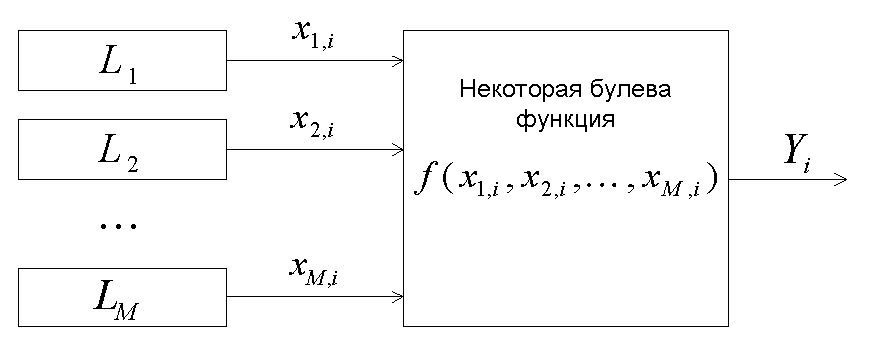
\includegraphics[width=0.7\textwidth]{pic/generators}
    \caption{Генератор с несколькими регистрами сдвига\label{fig:generators}}
\end{figure}

Таким образом, увеличение числа регистров сдвига с обратной связью увеличивает период последовательности. Однако более важным параметром для увеличения криптостойкости генератора является \emph{ длина регистра с линейной обратной связью}, эквивалентного по порождаемой последовательности. Такой эквивалентный регистр с линейной обратной связью находится с помощью алгоритма Берлекэмпа~---~Мэсси декодирования циклических кодов. В лучшем случае длина эквивалентного регистра соизмерима с периодом последовательности, порожденной нелинейным генератором. В общем случае определение эквивалентной длины является сложной задачей.


\subsection[Генераторы с нелинейными преобразованиями]{Генераторы с нелинейными \protect\\ преобразованиями}
\selectlanguage{russian}

Известно, что любая булева функция $f(x_1, x_2,  \ldots, x_M)$ может быть единственным образом записана многочленом Жегалкина\index{многочлен!Жегалкина}:
\[ \begin{array}{ll}
    f(x_1, x_2, \dots, x_M) & = ~c~ \oplus \\
    & \oplus \sum\limits_{1 \leq i \leq M} c_i x_i \oplus \\
    & \oplus \sum\limits_{1 \leq i < j \leq M} c_{i,j} x_i x_j \oplus \\
    & \oplus \sum\limits_{1 \leq i < j < k \leq M} c_{i,j,k} x_i x_j x_k \oplus \\
    & \oplus \ldots \oplus \\
    & \oplus ~ c_{1,2,\dots,M} ~ x_1 x_2 \dots x_M.
\end{array} \]

%Криптографу рекомендуется выбирать булеву функцию с возможно большим числом ненулевых коэффициентов при квадратичных членах полинома Жегалкина.

Второй способ улучшения криптостойкости последовательности поясняется с помощью рис.~\ref{fig:lfsr-zhegalkin}, на котором представлен регистр сдвига с $M$ ячейками и устройство, осуществляющее преобразование с помощью булевой функции $f(x_1, x_2, \dots, x_M)$, причем функция $f$ содержит нелинейные члены, то есть произведения $x_i x_j \dots$. Тактовый вход здесь такой же, как у регистров, показанных на других рисунках.

Если функция $f$ нелинейная, то в общем случае неизвестен полиномиальный алгоритм восстановления состояния регистров по нескольким последним выходам генератора. Таким образом, использование нескольких регистров сдвига увеличивает максимально возможный период по сравнению с одним регистром до $T < 2^{L_1 + L_2 + \dots + L_M}$, а нелинейность функции $f$ позволяет избежать простого нахождения состояния по выходу. Чтобы улучшить криптостойкость последовательности, порождаемой регистром, рекомендуется брать много нелинейных членов многочлена Жегалкина.

Такой подход применён в системе GPS. Удачных попыток ее взлома до сих пор нет.

\begin{figure}[!ht]
    \centering
	\includegraphics[width=0.4\textwidth]{pic/lfsr-zhegalkin}
    \caption{Криптографический генератор с нелинейной булевой функцией\label{fig:lfsr-zhegalkin}}
\end{figure}


\subsection[Мажоритарные генераторы, шифр A5/1]{Мажоритарные генераторы на примере алгоритма шифрования A5/1}\index{шифр!A5}
\selectlanguage{russian}

Третий способ улучшения криптостойкости последовательностей поясняется с помощью рис.~\ref{fig:gsm-a51-cipher}, на котором показан мажоритарный генератор ключей алгоритма потокового шифрования A5/1 стандарта GSM (GSM-2). В отличие от нелинейного комбинирования выходов нескольких регистров, применён условный сдвиг регистров, то есть на каждом такте некоторые регистры могут не сдвигаться, а оставаться в прежнем состоянии. На рисунке показана схема из трёх регистров сдвига с различными многочленами обратной связи (здесь применена обратная нумерация ячеек, коэффициентов и переменных по сравнению с предыдущими разделами):
\[ \left\{ \begin{array}{l}
    c_1(y) = y^{19} + y^{18} + y^{17} + y^{14} + 1, \\
    c_2(y) = y^{22} + y^{21} + 1, \\
    c_3(y) = y^{23} + y^{22} + y^{21} + y^8 + 1.
\end{array} \]

\begin{figure}[!ht]
    \centering
	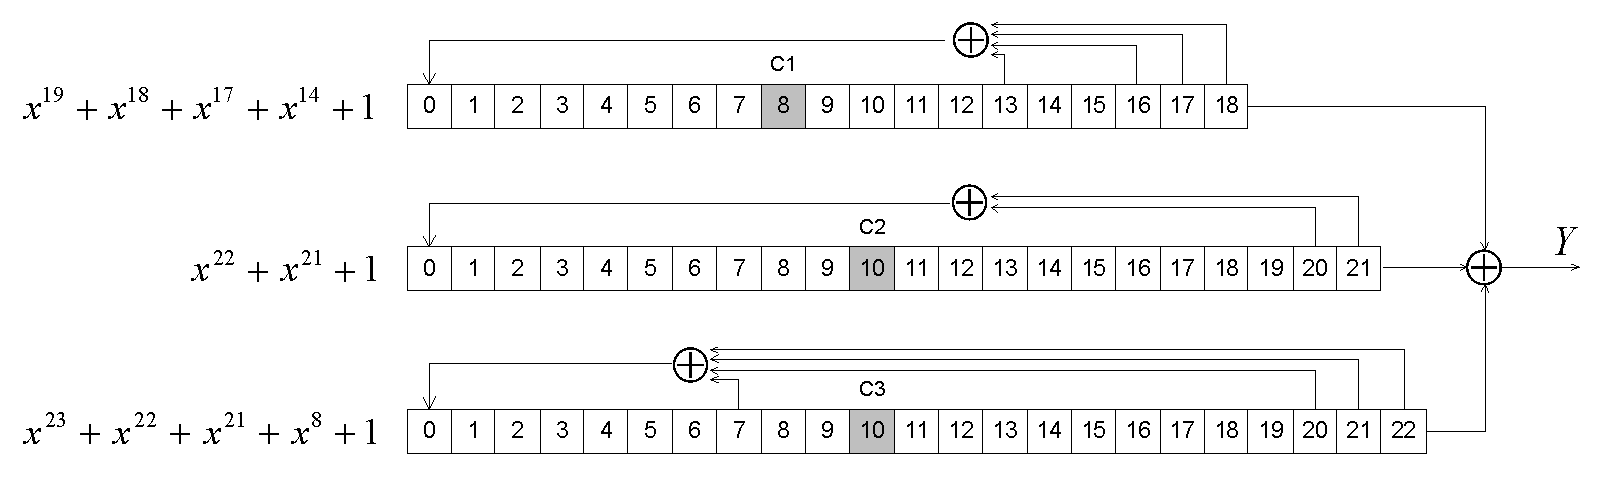
\includegraphics[width=\textwidth]{pic/gsm-a51-cipher}
    \caption{Регистр сдвига алгоритма шифрования A5/1\label{fig:gsm-a51-cipher}}
\end{figure}

В алгоритме A5/1 регистры сдвигаются не на каждом такте. Правило сдвига следующее. В каждом регистре есть один тактовый бит, определяющий сдвиг,  -- восьмой бит $\textrm{C1}$ для первого регистра, десятые биты $\textrm{C2}$ и $\textrm{C3}$ для второго и третьего регистров. На каждом такте вычисляется мажоритарное значение тактового бита $m = \textrm{majority}(\textrm{C1}, \textrm{C2}, \textrm{C3})$, т.~е. по большинству значений: 0 или 1. Если для данного регистра значение тактового бита совпадает с мажоритарным решением, то регистр сдвигается. Если не совпадает, то остаётся в прежнем состоянии без сдвига на следующий такт. Так как всего состояний тактовых битов $2^3$, то в среднем каждый регистр сдвигается в $\frac{3}{4}$ всех тактов.

Общее количество ячеек всех трёх регистров $19+22+23=64$, следовательно, период генератора A5/1 ~ $T < 2^{64}$. Данный шифр не может считаться стойким из-за возможности полного перебора. Например, известны атаки на шифр A5/1, требующие 150-300 GiB оперативной памяти и несколько минут вычислений одного ПК (2001 г.).



\chapter{Потоковые шифры}\label{chapter-stream-ciphers}
\selectlanguage{russian}

\section{Посимвольное шифрование}
\selectlanguage{russian}

Потоковые шифры осуществляют посимвольное шифрование открытого текста. Их основные достоинства: большая скорость шифрования по сравнению с блоковыми шифрами и относительно простая реализация.

Пусть имеется двоичная последовательность $x_{1} x_{2} \dots x_{N}$, представляющая открытый текст, и последовательность ключей $k_{1} k_{2} \dots k_{N}$. Шифрованная последовательность представляет собой сумму по модулю 2 этих двух последовательностей
\[ \begin{array}{l}
    y_{1} = x_{1} \oplus k_{1}, \\
    y_{2} = x_{2} \oplus k_{2}, \\
    \dots \\
    y_{N} = x_{N} \oplus k_{N}.
\end{array} \]

Если бы в двоичной последовательности ключей все символы были независимы, и нули и единицы равновероятны, то такая система по доказанному выше была бы совершенной, то есть обеспечивала бы независимость шифрованного текста от исходного текста и, как следствие, равенство нулю количества взаимной информации. Поэтому одна из основных задач при разработке систем потокового шифрования состоит в построении последовательностей с равномерным, случайным и независимым распределением.

Существует много способов построения двоичных последовательностей с распределением, близким к равномерному. Они называются псевдослучайными последовательностями\index{число!псевдослучайное}.

Пусть имеем некоторую двоичную последовательность $z_{1} z_{2} \ldots z_{N}$, полученную в результате подбрасывания <<неправильной монеты>> (монета считается неправильной, так как даёт неравномерное распределение). Когда выпадал герб, записывали символ $1$. Когда выпадала решка, записывали символ $0$. Чтобы теперь приблизить распределение к равномерному, преобразуем эту последовательность с помощью алгоритма Джона фон Неймана (John von Neumann). Разделим символы на пары. Если $z_{1} z_{2} = 11$ или $z_{1} z_{2} = 00$, то пара выбрасывается из последовательности; если $z_{1} z_{2} =10$, то записываем новый символ $u=1$; если $z_{1} z_{2} =01$, то записываем новый символ $u=0$. Получаем новую двоичную последовательность символов $u_{1}u_{2}\ldots $, у которой распределение нулей и единиц ближе к равномерному.
%(См. \textbf{Приложение 2}).


\section{Криптостойкие последовательности}\label{chapter-crypto-random}

Генераторы псевдослучайных чисел (ГПСЧ) ставят в соответствие набору символов $z_{1} z_{2} \dots z_{l}$ значение некоторой функции $f(z_{1} z_{2} \dots z_{l}) = f_{1}$. Следующим $l$ символам -- $f(z_{l+1} z_{l+2} \dots z_{2l}) = f_{2}$. Получают набор значений $f_{1} f_{2} \dots f_{N}$ и используют их в качестве случайной последовательности.

Для проверки степени близости к независимости и равномерному распределению символов существует набор тестов. Американский институт стандартизации NIST разработал 16 тестов на псевдослучайность. Подсчитывается число нулей и единиц, число одинаковых соседних пар, число одинаковых подпоследовательностей, автокорреляция, частота следующего символа в зависимости от предыдущих и т.д. Вычисляют вероятность символа 0 (или 1)
\[
    P(f_i = 0 | f_{i-1} f_{i-2} \dots f_{i-k}) = \frac{1}{2} - \epsilon.
\]
Если вычисления осуществляются за полиномиальное время от длины подпоследовательности $k$, то есть с количеством битовых операций $O(k^{\textrm{const}})$, то тест называют \emph{полиномиальным}\index{задача!полиномиальная}.

Псевдослучайная последовательность удовлетворяет \textbf{тесту <<следующего бита>>}, если не существует полиномиального по $k$ теста, позволяющего по предыдущим $k$ битам определить следующий бит с вероятностью, отличной от $\frac{1}{2} - \epsilon$, принимая во внимание погрешность оценки $\epsilon$. Последовательность, удовлетворяющая тесту <<следующего бита>>, также удовлетворяет всем возможным полиномиальным тестам по $k$ на равномерность распределения, и наоборот.

Последовательность называется \emph{криптографически стойкой} или \emph{криптостойкой}, если она удовлетворяет тесту <<следующего бита>>.

\subsection{Генератор BBS}
\selectlanguage{russian}

Имеются примеры <<хороших>> генераторов, вырабатывающих криптографически стойкие последовательности, например генератор \textbf{Blum-Blum-Shub (BBS)}. Алгоритм работы состоит в следующем. Выбирают большие (длиной не менее 512 бит) простые числа\index{число!простое} $p, q$, которые при делении на $4$ дают в остатке $3$. Вычисляют $n = p q$. С помощью генератора случайных чисел вырабатывают число $x_{0}$, где $1 \leq x_0 \leq n-1$ и $\gcd(x_0, n) = 1$. Далее проводят следующие вычисления:
\[ \begin{array}{l}
        x_{1} = x_{0}^{2} \mod n,\\
        x_{2} = x_{1}^{2} \mod n,\\
        \dots\\
        x_{N} = x_{N-1}^{2} \mod n.
\end{array} \]

Для каждого вычисленного значения оставляют один младший разряд. Вычисляют двоичную псевдослучайную последовательность $k_1, k_2, k_3, \dots$:
\[ \begin{array}{l}
        k_{1} = x_{1} \mod 2,\\
        k_{2} = x_{2} \mod 2,\\
        \dots \\
        k_{N} = x_{N} \mod 2.
\end{array} \]

Число $a$ называется \emph{квадратичным вычетом} по модулю $n$, если для него существует квадратный корень $b$ (или два корня): $a = b^2 \mod n$. Для $p,q ~=~ 3 \mod 4$ верно утверждение, что квадратичный вычет имеет единственный корень, и операция $x \rightarrow x^2 \mod n$, применённая к элементам множества всех квадратичных вычетов $\set{QR}_n$ по модулю $n$, является перестановкой множества $\set{QR}_n$.

Полученная последовательность квадратичных вычетов $x_1, x_2, x_3, \dots$ -- периодическая с периодом $T < |\set{QR}_n|$. Чтобы ее период для случайного $x_0$ с большой вероятностью оказался большим, числа $p,q$ выбирают с условием малого $\gcd(\varphi(p-1), \varphi(q-1))$, где $\varphi(n)$ -- функция Эйлера.

Полученная последовательность ключей является криптографически стойкой. Доказано, что для <<взлома>> (т.~е. определения следующего символа с вероятностью, отличной от $\frac{1}{2}$) требуется разложить число $n=pq$ на множители. Разложение числа на множители считается трудной задачей, все известные алгоритмы не являются полиномиальными по $\log_2 n$.

Оказывается, что если вместо одного последнего бита $k_i = x_i \mod 2$ брать $O(\log_2 \log_2 n)$ последних бит рассмотренного выше генератора $x_i$, то полученная последовательность останется криптостойкой.

Большим недостатком генератора BBS является малая скорость генерирования бит.


%\subsection{Генератор Микали}\index{генератор!Микали}

Другой пример -- генератор Микали.

Так же выбирают большие простые числа $p,q$ с битовой длиной не менее 512, вычисляют число $n = pq$. Находят функцию Эйлера $\varphi(n) = (p-1) (q-1)$ и задают целое число $e$, такое, что наибольший общий делитель $\gcd(e, \varphi(n)) = 1$. С помощью датчика случайных чисел выбирают $0 \leq x_{0} \leq n-1$. Вычисляют
\[ \begin{array}{l}
    x_1 = x_0^e \mod n, \\
    x_2 = x_1^e \mod n, \\
    \dots \\
    x_N = x_{N-1}^e \mod n.
\end{array} \]
Чтобы уменьшить сложность вычислений, в значениях $x_i$ оставляют $l$ младших разрядов, причем $l \leq \log_2 \log_2 N$. Последовательность ключей получают в виде
\[ \begin{array}{l}
    k_1 = x_1^2 \mod 2, \\
    k_2 = x_2^2 \mod 2, \\
    \dots \\
    k_N = x_N^2 \mod 2. \\
\end{array} \]

Как и генератор BBS, генератор Микали -- криптостойкий, для его взлома требуется разложить число $n$ на множители. Недостаток -- маленькая скорость.


\section{Последовательности максимального периода}
\selectlanguage{russian}
\label{section:max-seq}

Периодические последовательности с максимальным периодом называются $M$-последовательностями\index{$M$-последовательность} и характеризуются идеальной функцией автокорреляции.

Пусть $M$-последовательность имеет вид $x_1, x_2, \dots, x_n$, где значения $x_{i} = \pm 1$. Функция автокорреляции\index{функция!автокорреляции} такой последовательности имеет вид
\[
    \sum\limits_{i=1}^{T} x_i x_{i + \tau}  = \left\{ \begin{array}{rcl}
        -1,\ \tau&\neq& 0, \\
        T,\ \tau&=& 0. \\
    \end{array} \right.
\]

$M$-последовательности можно генерировать с помощью регистров сдвига с линейной обратной связью. На рис.~\ref{fig:impulse} показан регистр сдвига, состоящий из ячеек памяти со входами для информационных символов и тактовых импульсов. На рис.~\ref{fig:generator} тактовые импульсы опущены. Через $S_{j}$ обозначено содержимое $j$-й ячейки, где $j=\overline{0,L-1}$. В цепь обратной связи введены сумматоры по модулю 2 и умножители с коэффициентами $c_{j}$, принимающими значения $0,1$. Поступление тактового импульса вызывает сдвиг в регистре сдвига.
\begin{figure}[!ht]
	\centering
    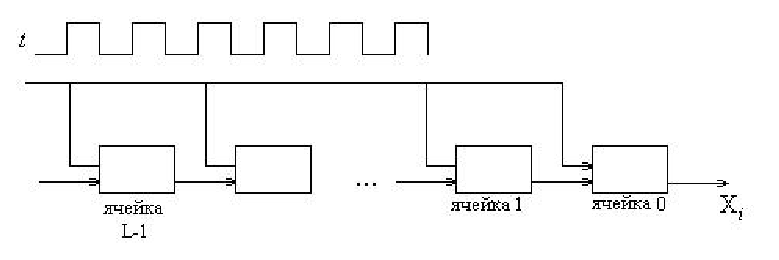
\includegraphics[width=0.8\textwidth]{pic/taktovi-impuls}
    \caption{Тактовые импульсы\label{fig:impulse}}
\end{figure}

В этой схеме используется линейная обратная связь. Выход ячейки с номером $L-1$ умножают на $c_{1}$, выход следующей ячейки $L-2$ умножают на $c_2$ и так далее. После умножения выходы ячеек суммируют по модулю 2 и результат подают на вход крайней ячейки $(L-1)$. Если содержимое всех ячеек состоит из нулей, то генерируемая последовательность также состоит из одних нулей. Если имеется ненулевое заполнение $S_{j-1}, S_{j-2}, \dots, S_{j-L}$, то после поступления $j$-го тактового импульса имеем сигнал на выходе такой, как показано на рис.~\ref{fig:generator}:
\begin{figure}[!ht]
	\centering
	\includegraphics[width=0.8\textwidth]{pic/generator}
    \caption{Генератор\label{fig:generator}}
\end{figure}

Во всем разделе~\ref{section:max-seq}  операцией <<$+$>>  обозначается операция сложения двоичных коэффициентов и многочленов по модулю 2.
\[
    S_{j} = c_{1} S_{j-1} + c_{2} S_{j-2} +  \dots  + c_{L-1} S_{j-L+1} + c_{L} S_{j-L}.
\]

Это соотношение определяет принцип работы генератора на регистрах сдвига\index{регистр сдвига}. Всего $2^{L}$ начальных условий, задающих значения бит в ячейках, из них $2^{L}-1$ ненулевых начальных условий. Генерируемая двоичная последовательность является периодической с периодом $T\leq 2^{L}-1$. Величина периода зависит от коэффициентов обратной связи $c_{1},  \ldots, c_{L} $.

Набор коэффициентов задаётся многочленом обратной связи
    \[ c(y) = 1 + c_1 y+ c_2 y^2 + \dots + c_L y^L. \]
Свойства этого многочлена влияют на период генерируемой последовательности. Рассмотрим его подробнее.

Многочлен $c(y)$ над полем $\GF{2}$ с коэффициентами $c_i \in \GF{2}$ называется \textit{приводимым}, если его можно представить в виде произведения многочленов меньшей степени. Например, многочлен $1 + y^{2} = (1 + y) (1 + y) = 1 + y + y + y^2 = 1 + y^2$ является приводимым. Многочлен $1 + y + y^{2}$ -- неприводимый.

Приведём без доказательства два важных утверждения.
\begin{itemize}
    \item Пусть $c(y)$ -- неприводимый многочлен. Тогда существует такое значение $m$, что $y^{m} + 1$ делится без остатка на $c(y)$, то есть $\frac{y^{m} + 1}{c(y)} = d(y)$.
    \item Существуют многочлены $c(y)$, для которых $m=2^{L} - 1$, где L -- степень многочлена $c(y)$. Эти многочлены называются примитивными.
\end{itemize}

Если $c(y)$ -- примитивный многочлен\index{многочлен!примитивный}, то период генерируемой последовательности является максимальным, то есть равным $T = 2^{L} - 1$. Генерируемые последовательности являются $M$-последовательностями, то есть последовательностями максимального периода. Для любого начального ненулевого состояния генерируется циклический сдвиг одной и той же последовательности максимального периода $T=2^{L} - 1$.

Оказывается, что многочлен обратной связи и состояние регистра определяются однозначно по $2L$ последовательным символам выхода регистра сдвига с линейной обратной связью (с помощью алгоритма Берлекэмпа~---~Мэсси или алгоритма Евклида).

Например, в спутниках GPS имеется регистр сдвига c 43 ячейками и периодом генерируемой последовательности $2^{43} - 1$. Длительность одного импульса $\sim 0{,}1$ мкс, период последовательности примерно равен одному году. Если бы для генерирования криптостойкой последовательности был просто применён регистр сдвига с линейной обратной связью (РСЛОС), то, чтобы найти многочлен обратной связи, криптоаналитику достаточно было бы получить 86 символов последовательности.

Чтобы РСЛОС можно было использовать в качестве составной части криптографически стойкого генератора псевдослучайной последовательности или поточного шифра, создатели криптографических примитивов комбинируют несколько регистров сдвига, в том числе с помощью приводимых далее способов.


\section[Три способа улучшения последовательностей]{Три способа улучшения \protect\\ последовательностей}

\subsection[Генераторы с несколькими регистрами сдвига]{Генераторы с несколькими регистрами \protect\\ сдвига}
\selectlanguage{russian}

Первый способ улучшения криптографических свойств последовательности состоит в создании композиционных генераторов из нескольких регистров сдвига при определённом способе выбора параметров. Схема такого генератора показана на рис.~\ref{fig:generators}. Здесь $L_i, ~ i = 1, 2, \dots, M$ -- регистры сдвига с линейной обратной связью. Вырабатываемые ими двоичные символы $x_{1,i}, x_{2,i},  \dots, x_{M,i}$ поступают синхронно на устройство преобразования, задаваемое булевой функцией $f(x_{1,i}, x_{2,i}, \dots, x_{M,i})$. В булевой функции аргументы принимают значения $0,1$ и значения функции также $0,1$.

Число ячеек в $i$-м регистре равно $L_{i}$, причем $\gcd(L_i, L_j)=1$ для $i \neq j$, где  $\gcd$ -- наибольший общий делитель. Общее число ячеек $L = \sum\limits_{i=1}^M L_i$. Булева функция $f$ должна включать слагаемое по одному из входов, т.~е. $f = \ldots + x_i + \ldots$, для того чтобы двоичные символы на выходе этой функции были равновероятными. Период этого генератора может достигать величины (немного меньше)
    \[ T \simeq 2^L. \]

\begin{figure}[!ht]
	\centering
	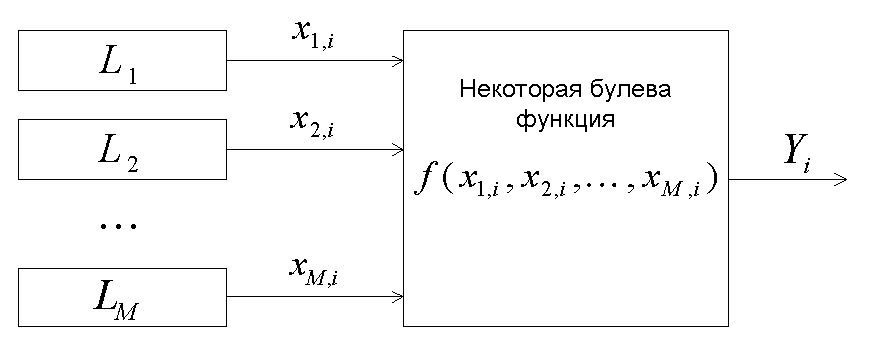
\includegraphics[width=0.7\textwidth]{pic/generators}
    \caption{Генератор с несколькими регистрами сдвига\label{fig:generators}}
\end{figure}

Таким образом, увеличение числа регистров сдвига с обратной связью увеличивает период последовательности. Однако более важным параметром для увеличения криптостойкости генератора является \emph{ длина регистра с линейной обратной связью}, эквивалентного по порождаемой последовательности. Такой эквивалентный регистр с линейной обратной связью находится с помощью алгоритма Берлекэмпа~---~Мэсси декодирования циклических кодов. В лучшем случае длина эквивалентного регистра соизмерима с периодом последовательности, порожденной нелинейным генератором. В общем случае определение эквивалентной длины является сложной задачей.


\subsection[Генераторы с нелинейными преобразованиями]{Генераторы с нелинейными \protect\\ преобразованиями}
\selectlanguage{russian}

Известно, что любая булева функция $f(x_1, x_2,  \ldots, x_M)$ может быть единственным образом записана многочленом Жегалкина\index{многочлен!Жегалкина}:
\[ \begin{array}{ll}
    f(x_1, x_2, \dots, x_M) & = ~c~ \oplus \\
    & \oplus \sum\limits_{1 \leq i \leq M} c_i x_i \oplus \\
    & \oplus \sum\limits_{1 \leq i < j \leq M} c_{i,j} x_i x_j \oplus \\
    & \oplus \sum\limits_{1 \leq i < j < k \leq M} c_{i,j,k} x_i x_j x_k \oplus \\
    & \oplus \ldots \oplus \\
    & \oplus ~ c_{1,2,\dots,M} ~ x_1 x_2 \dots x_M.
\end{array} \]

%Криптографу рекомендуется выбирать булеву функцию с возможно большим числом ненулевых коэффициентов при квадратичных членах полинома Жегалкина.

Второй способ улучшения криптостойкости последовательности поясняется с помощью рис.~\ref{fig:lfsr-zhegalkin}, на котором представлен регистр сдвига с $M$ ячейками и устройство, осуществляющее преобразование с помощью булевой функции $f(x_1, x_2, \dots, x_M)$, причем функция $f$ содержит нелинейные члены, то есть произведения $x_i x_j \dots$. Тактовый вход здесь такой же, как у регистров, показанных на других рисунках.

Если функция $f$ нелинейная, то в общем случае неизвестен полиномиальный алгоритм восстановления состояния регистров по нескольким последним выходам генератора. Таким образом, использование нескольких регистров сдвига увеличивает максимально возможный период по сравнению с одним регистром до $T < 2^{L_1 + L_2 + \dots + L_M}$, а нелинейность функции $f$ позволяет избежать простого нахождения состояния по выходу. Чтобы улучшить криптостойкость последовательности, порождаемой регистром, рекомендуется брать много нелинейных членов многочлена Жегалкина.

Такой подход применён в системе GPS. Удачных попыток ее взлома до сих пор нет.

\begin{figure}[!ht]
    \centering
	\includegraphics[width=0.4\textwidth]{pic/lfsr-zhegalkin}
    \caption{Криптографический генератор с нелинейной булевой функцией\label{fig:lfsr-zhegalkin}}
\end{figure}


\subsection[Мажоритарные генераторы, шифр A5/1]{Мажоритарные генераторы на примере алгоритма шифрования A5/1}\index{шифр!A5}
\selectlanguage{russian}

Третий способ улучшения криптостойкости последовательностей поясняется с помощью рис.~\ref{fig:gsm-a51-cipher}, на котором показан мажоритарный генератор ключей алгоритма потокового шифрования A5/1 стандарта GSM (GSM-2). В отличие от нелинейного комбинирования выходов нескольких регистров, применён условный сдвиг регистров, то есть на каждом такте некоторые регистры могут не сдвигаться, а оставаться в прежнем состоянии. На рисунке показана схема из трёх регистров сдвига с различными многочленами обратной связи (здесь применена обратная нумерация ячеек, коэффициентов и переменных по сравнению с предыдущими разделами):
\[ \left\{ \begin{array}{l}
    c_1(y) = y^{19} + y^{18} + y^{17} + y^{14} + 1, \\
    c_2(y) = y^{22} + y^{21} + 1, \\
    c_3(y) = y^{23} + y^{22} + y^{21} + y^8 + 1.
\end{array} \]

\begin{figure}[!ht]
    \centering
	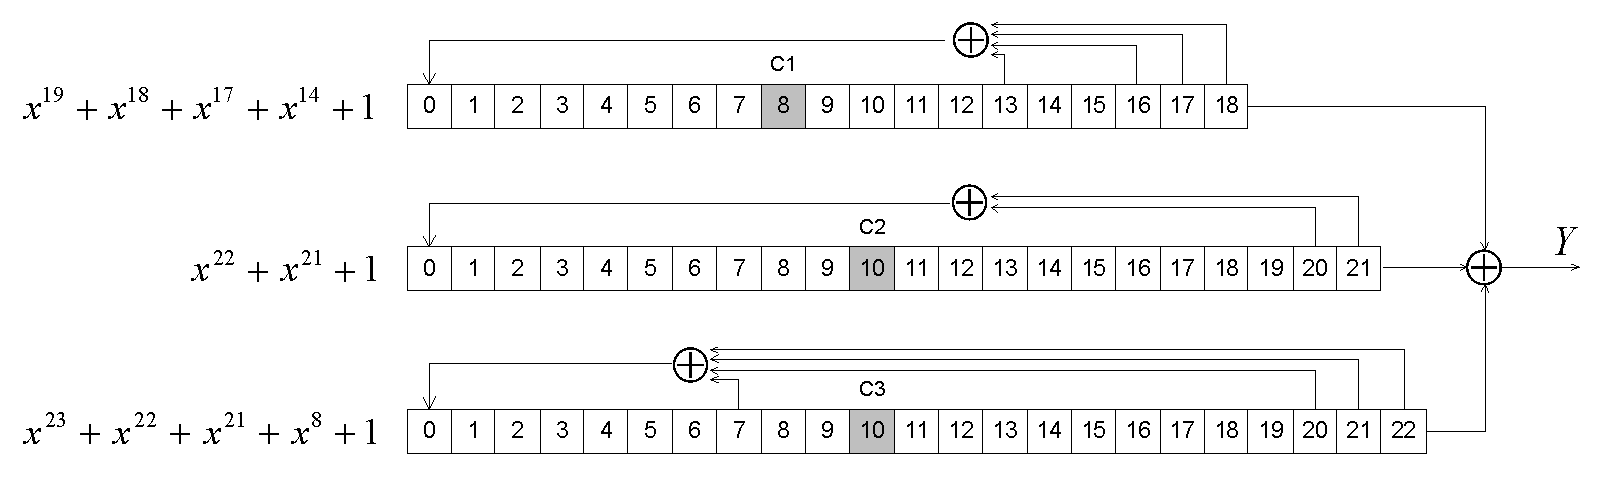
\includegraphics[width=\textwidth]{pic/gsm-a51-cipher}
    \caption{Регистр сдвига алгоритма шифрования A5/1\label{fig:gsm-a51-cipher}}
\end{figure}

В алгоритме A5/1 регистры сдвигаются не на каждом такте. Правило сдвига следующее. В каждом регистре есть один тактовый бит, определяющий сдвиг,  -- восьмой бит $\textrm{C1}$ для первого регистра, десятые биты $\textrm{C2}$ и $\textrm{C3}$ для второго и третьего регистров. На каждом такте вычисляется мажоритарное значение тактового бита $m = \textrm{majority}(\textrm{C1}, \textrm{C2}, \textrm{C3})$, т.~е. по большинству значений: 0 или 1. Если для данного регистра значение тактового бита совпадает с мажоритарным решением, то регистр сдвигается. Если не совпадает, то остаётся в прежнем состоянии без сдвига на следующий такт. Так как всего состояний тактовых битов $2^3$, то в среднем каждый регистр сдвигается в $\frac{3}{4}$ всех тактов.

Общее количество ячеек всех трёх регистров $19+22+23=64$, следовательно, период генератора A5/1 ~ $T < 2^{64}$. Данный шифр не может считаться стойким из-за возможности полного перебора. Например, известны атаки на шифр A5/1, требующие 150-300 GiB оперативной памяти и несколько минут вычислений одного ПК (2001 г.).



\subimport*{hash-functions/}{index}

\subimport*{public-key/}{index}

\subimport*{protocols/}{index}

\subimport*{secret-sharing/}{index}

\subimport*{secure-systems-examples/}{index}

\subimport*{user-authentication/}{index}

\subimport*{software-security/}{index}

%\chapter{Послесловие}
%Это должно быть что-то в виде заключения, объяснения, почему именно эти темы выбраны, насколько актуален материал с теоретической и практической точки зрения.

\subimport*{appendix/}{index}

\printindex

\printusedliterature

\end{document}
